% Copyright (c) 2014,2016 Casper Ti. Vect
\chapter{系統詳細設計與實現}
在前章中已將本文的系統設計概要架構說明,在本章中將對數據庫的內容信息設計進行詳細的說明、數據庫ER模型架構、各個模塊的類與類之間的關係、每個模塊運作的順序以及模塊與模塊之間的響應關係,最後則是系統實現的平台展示。

	\section{BTMS數據庫設計}

	比特幣的交易監督系統應用了六個信息表,分別為商家信息、產品信息、交易信息、用戶信息、職工信息以及商家產品信息,以下將逐一說明:

		\begin{figure}[!htbp]
			\centering
			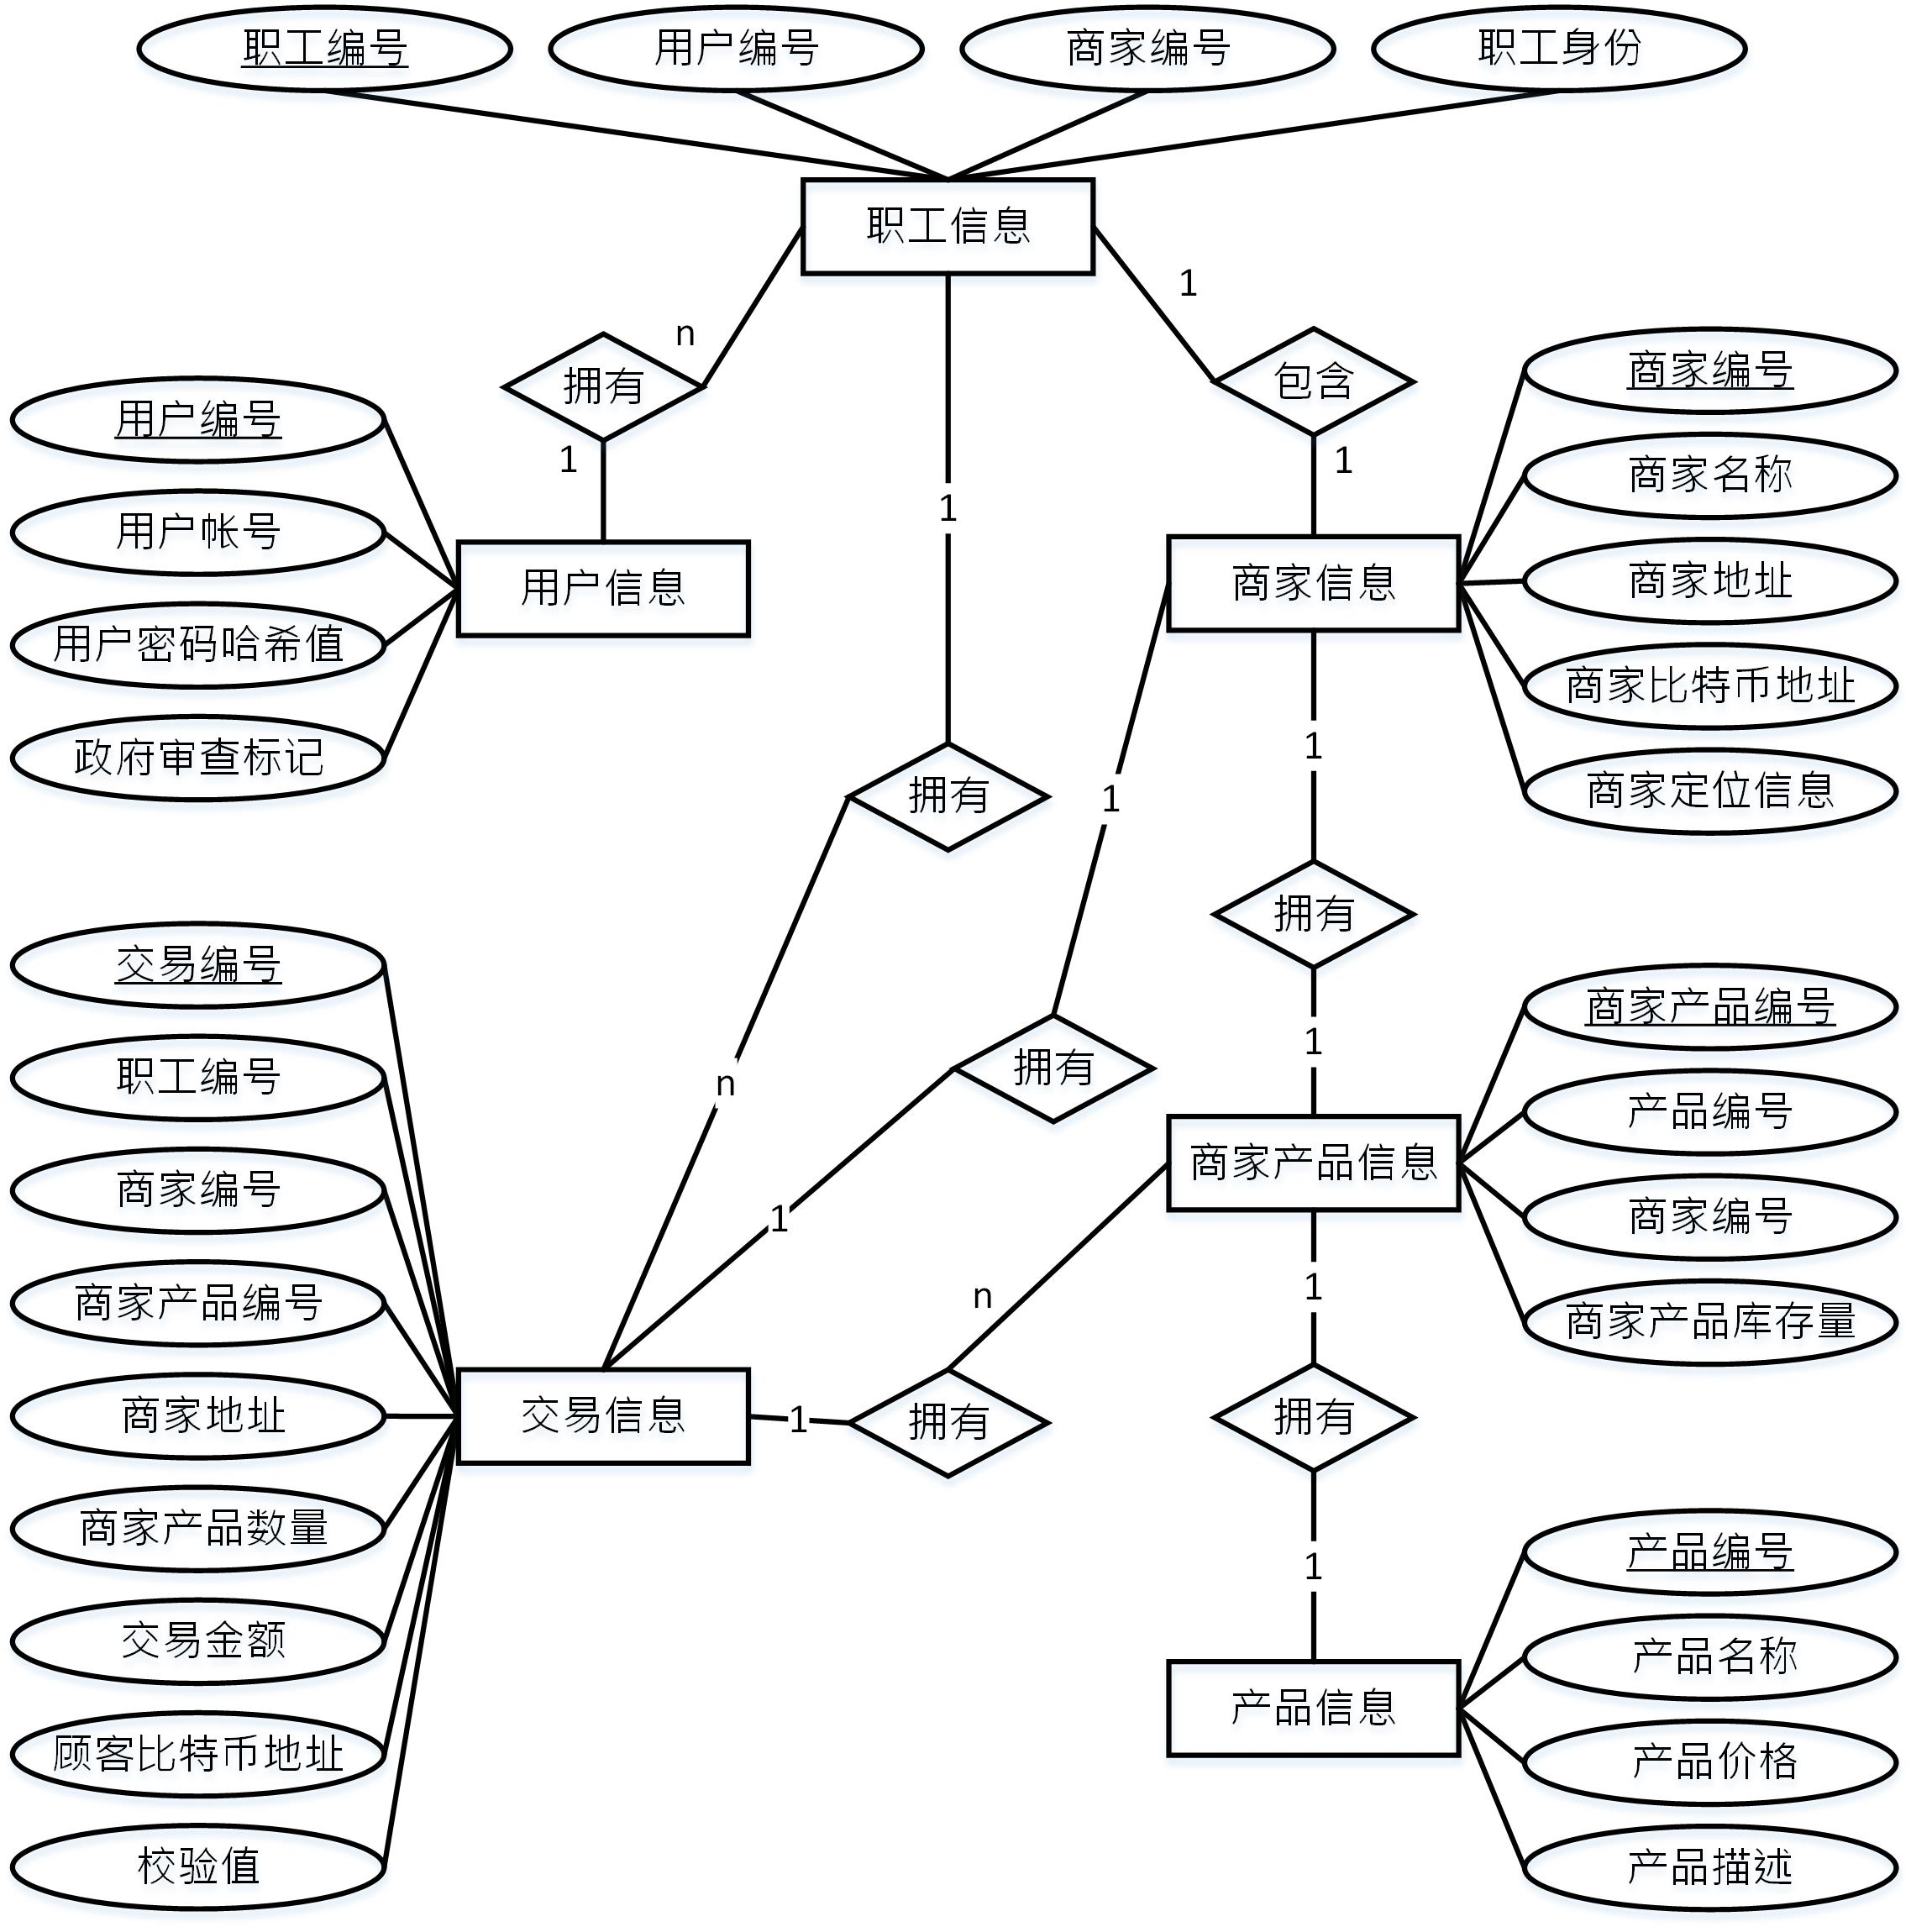
\includegraphics[width = 0.9\textwidth]{er.jpg}
			\caption{BTMS數據庫實體關係圖}\label{db}
		\end{figure}

		\begin{enumerate}
		\item 商家信息表:存儲正在審核中的企業信息或已經過審核的企業信息。表\ref{store}存儲的信息包括商家編號、商家名稱、商家地址、商家比特幣地址以及商家定位信息。


				\begin{table}[!htbp]
				\centering
				\caption{商家信息表}
				\label{store}
				\resizebox{\textwidth}{!}{%
				\begin{tabular}{|c|c|c|c|c|c|}
				\hline
				序號 & 字段名 & 字段說明 & 類型 & 是否為空 & 主外鍵 \\ \hline
				1 & STORE\_ID & 商家編號 & int & 否 & PK \\ \hline
				2 & STORE\_NAME & 商家名稱 & navarchar(20) & 否 &  \\ \hline
				3 & STORE\_ADDRESS & 商家地址 & navarchar(50) & 否 &  \\ \hline
				4 & STORE\_BTCADDRESS & 商家比特幣地址 & navarchar(50) & 否 &  \\ \hline
				5 & STORE\_GPS & 商家定位信息 & navarchar(30) & 否 &  \\ \hline
				\end{tabular}%
				}
				\end{table}

		\item 產品信息表:只有授權用戶才能登錄添加或修改交易產品信息。表\ref{product}產品信息表內容包括產品編號、產品名稱、產品價格以及產品描述信息。

				\begin{table}[!htbp]
				\centering
				\caption{產品信息表}
				\label{product}
				
				\begin{tabular}{|c|c|c|c|c|c|}
				\hline
				序號 & 字段名 & 字段說明 & 類型 & 是否為空 & 主外鍵 \\ \hline
				1 & PRODUCT\_ID & 產品編號 & int & 否 & PK \\ \hline
				2 & PRODUCT\_NAME & 產品名稱 & navarchar(10) & 否 &  \\ \hline
				3 & PRODUCT\_PRICE & 產品價格 & float & 否 &  \\ \hline
				4 & PRODUCT\_DESCRIPTION & 產品描述 & navarchar(50) & 是 &  \\ \hline
				\end{tabular}
				\end{table}

		\item 交易信息表:表\ref{tx}記錄包括交易編號、職工編號、商家編號、商家產品編號、商家地址、商家產品數量、交易金額、顧客比特幣地址和最後確認字段的校驗值。

				% \usepackage{graphicx}
				\begin{table}[!htbp]
				\centering
				\caption{交易信息表}
				\label{tx}
				\resizebox{\textwidth}{!}{%
				\begin{tabular}{|c|c|c|c|c|c|}
				\hline
				序號 & 字段名 & 字段說明 & 類型 & 是否為空 & 主外鍵 \\ \hline
				1 & TX\_ID & 交易編號 & int & 否 & PK \\ \hline
				2 & STAFF\_ID & 職工編號 & int & 否 & FK \\ \hline
				3 & STORE\_ID & 商家編號 & int & 否 & FK \\ \hline
				4 & STOREPRODUCT\_ID & 商家產品編號 & int & 否 & FK \\ \hline
				5 & STORE\_ADDRESS & 商家地址 & navarchar(50) & 否 & FK \\ \hline
				6 & STOREPRODUCT\_QUANTITY & 商家產品數量 & int & 否 &  \\ \hline
				7 & TX\_AMOUNT & 交易金額 & float & 否 &  \\ \hline
				8 & CONSUMER\_BTCADDRESS & 顧客比特幣地址 & navarchar(50) & 否 &  \\ \hline
				9 & CHECK & 校驗值 & bool & 否 &  \\ \hline
				\end{tabular}%
				}
				\end{table}

		\item 用戶信息表:表\ref{user}存儲所有用戶信息,包括政府、商家及顧客之個人的帳戶編號與帳號,而用戶密碼則以哈希值的方式保存以增加用戶安全性,最後則是政府審查值,倘若通過為"1",未通過為"0"。

				\begin{table}[!htbp]
				\centering
				\caption{用戶信息表}
				\label{user}
				\resizebox{\textwidth}{!}{%
				\begin{tabular}{|c|c|c|c|c|c|}
				\hline
				序號 & 字段名 & 字段說明 & 類型 & 是否為空 & 主外鍵 \\ \hline
				1 & USER\_ID & 用戶編號 & int & 否 & PK \\ \hline
				2 & USER\_ACCOUNT & 用戶帳號 & navarchar(30) & 否 &  \\ \hline
				3 & USER\_PASSWORDHASH & 用戶密碼哈希值 & navarchar(30) & 否 &  \\ \hline
				4 & GOVT\_AUTH & 政府審查 & bool & 否 &  \\ \hline
				\end{tabular}
				}
				\end{table}

		\item 職工信息表:表\ref{staff}信息表存儲各個商家擁有的職工信息,包括各職工編號、用戶編號、商家編號及職工身份。
				\begin{table}[!htbp]
				\centering
				\caption{職工信息表}
				\label{staff}
				\begin{tabular}{|c|c|c|c|c|c|}
				\hline
				序號 & 字段名 & 字段說明 & 類型 & 是否為空 & 主外鍵 \\ \hline
				1 & STAFF\_ID & 職工編號 & int & 否 & PK \\ \hline
				2 & USER\_ID & 用戶編號 & int & 否 & FK \\ \hline
				3 & STORE\_ID & 商家編號 & int & 否 & FK \\ \hline
				4 & STAFF\_STATUS & 職工身份 & navarchar(20) & 否 &  \\ \hline
				\end{tabular}
				\end{table}

		\item 商家產品信息表:表\ref{storeproduct}存儲各家商家當前商家產品存貨信息,由商家產品編號、產品編號、商家編號及商家產品庫存量所組成。
				\begin{table}[!htbp]
				\centering
				\caption{商家產品信息表}
				\label{storeproduct}
				\begin{tabular}{|c|c|c|c|c|c|}
				\hline
				序號 & 字段名 & 字段說明 & 類型 & 是否為空 & 主外鍵 \\ \hline
				1 & STOREPRODUCT\_ID & 商家產品編號 & int & 否 & PK \\ \hline
				2 & PRODUCT\_ID & 產品編號 & int & 否 & FK \\ \hline
				3 & STORE\_ID & 商家編號 & int & 否 & FK \\ \hline
				4 & STOREPRODUCT\_INVENTORY & 商家產品庫存量 & int & 否 &  \\ \hline
				\end{tabular}
				\end{table}

	\end{enumerate}

\section{系統模塊設計}
在本系統中共有三種用戶,分別為顧客、商家以及職工,首先是用戶註冊與登入模塊,其餘總共有四個管理模塊分別為商家產品管理模塊、職工管理模塊、商家交易管理模塊和顧客交易管理模塊,以下將說明各個模塊類圖設計以及時序圖運作。

\subsubsection{(一)用戶註冊與登入模塊}
在本系統中僅職工與商家需要進行註冊,並且需要經過政府的審查批准。職工與商家皆為用戶,皆可使用用戶註冊模塊。圖\ref{c3}為用戶註冊與登入模塊類圖,在LoginManagement類當中分別需要調用RegistNewUser類實現用戶註冊以及LoginUser類實現用戶登入。RegistNewUser類中hash()方法是將用戶輸入的用戶密碼使用哈希算法生成用戶密碼哈希值,addnewuser()方法則是將用戶帳號和密碼傳送至User類。在LoginUser類中getuserpasswordhash()方法是向User類取得該用戶帳號的密碼哈希值。

	\begin{figure}[!htbp]
		\centering
		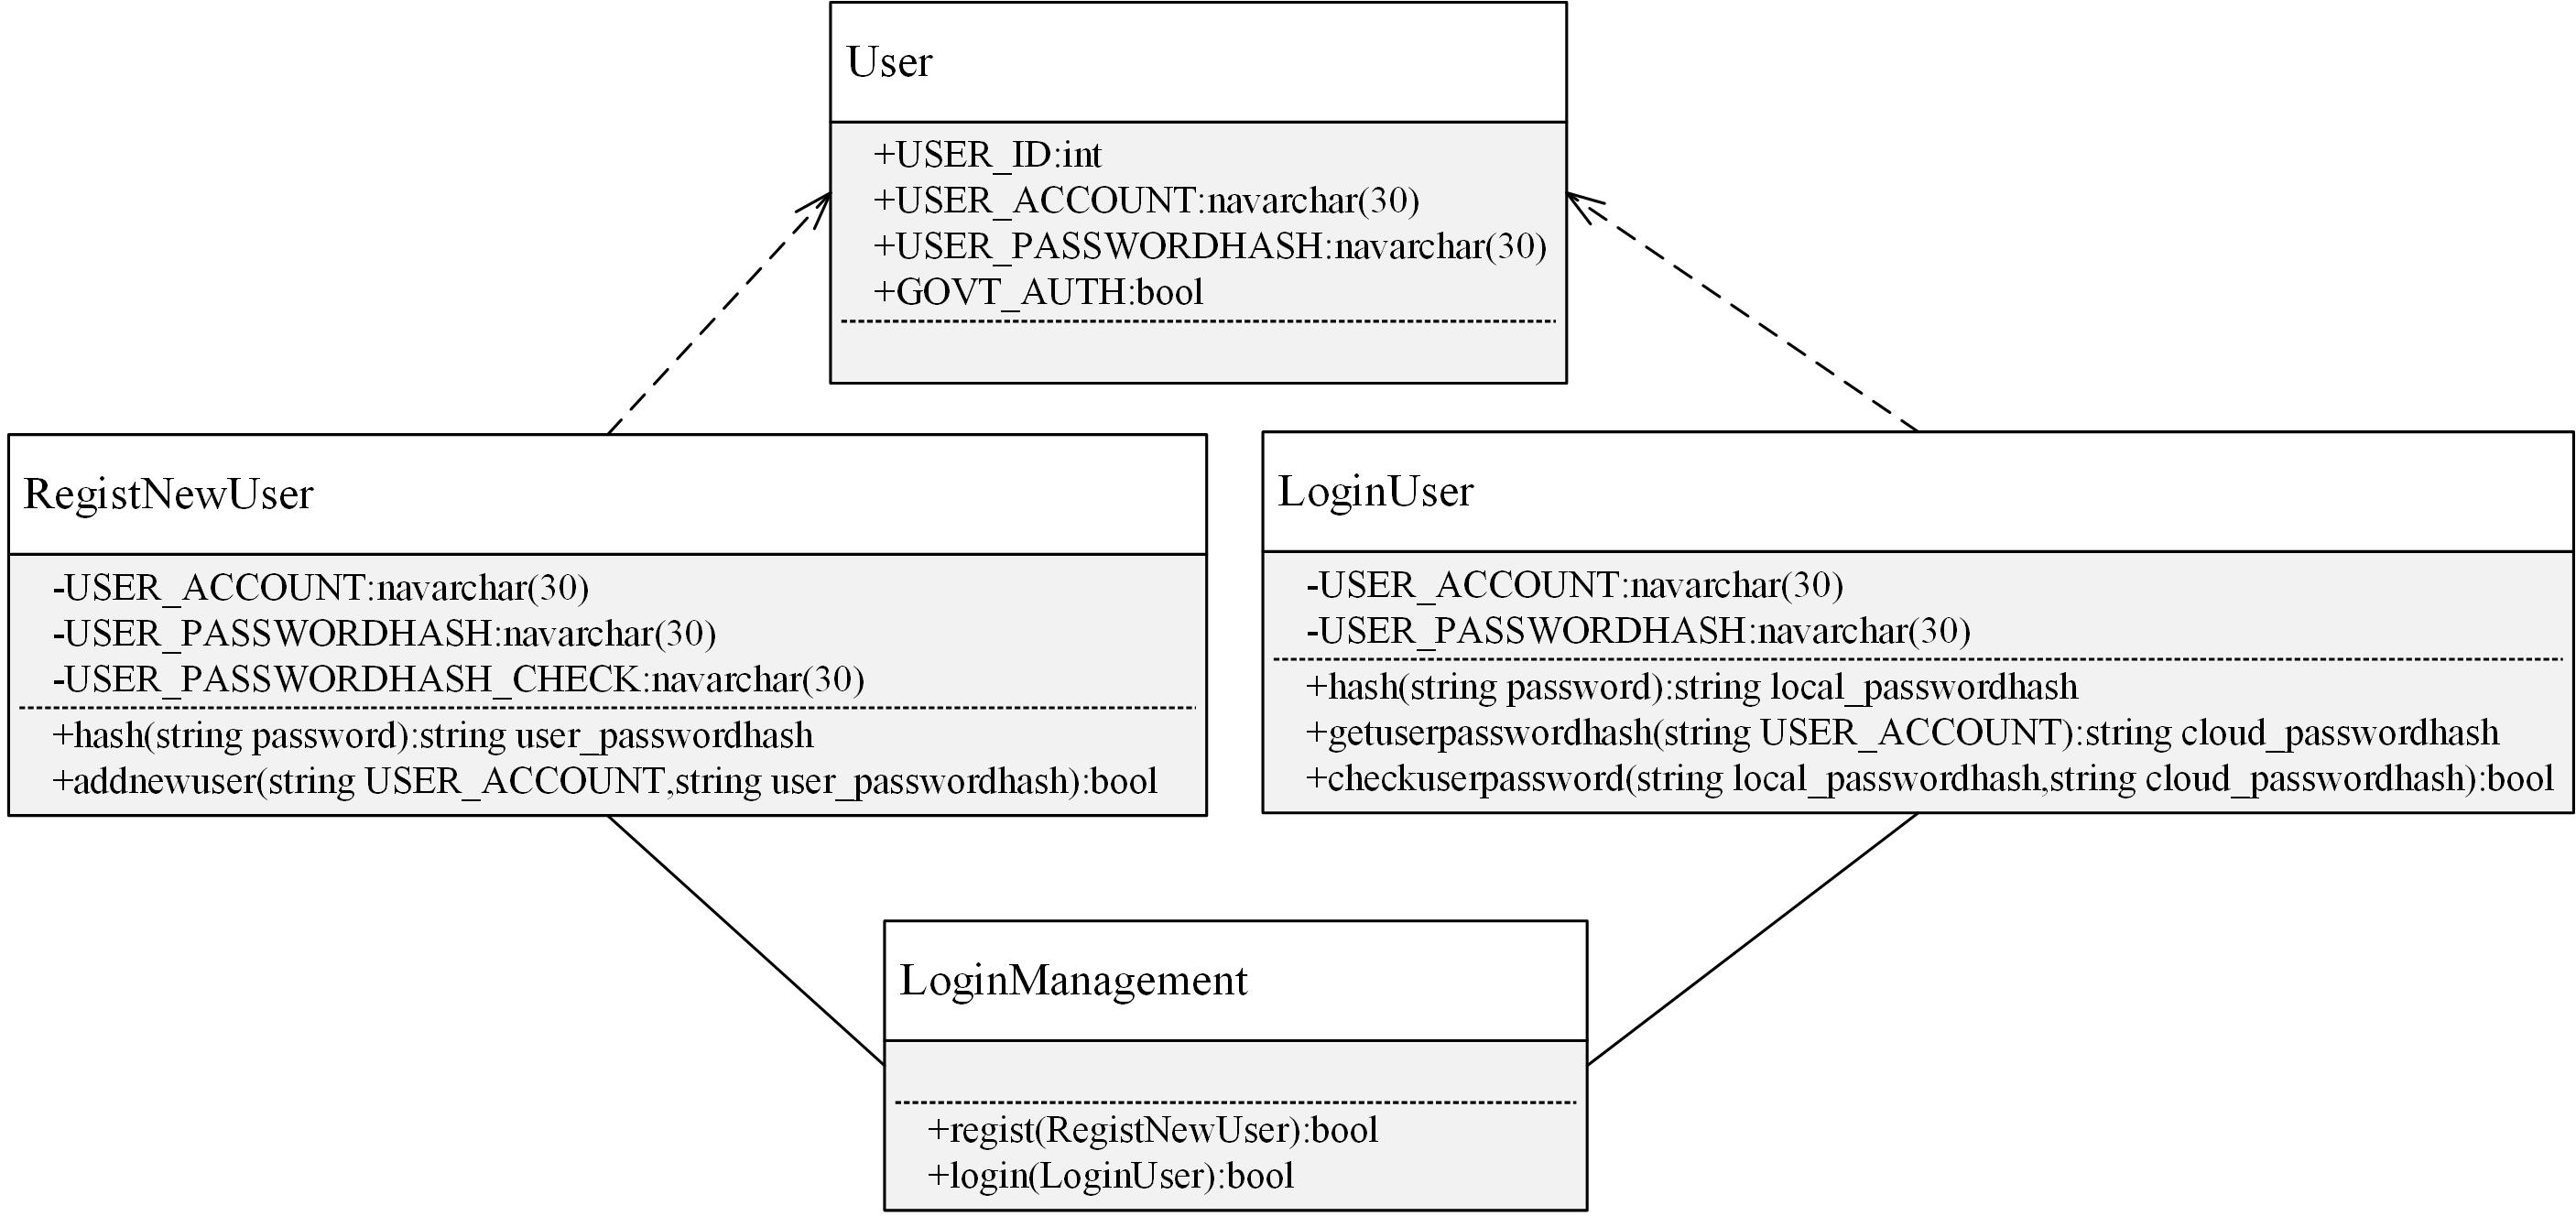
\includegraphics[width = 0.9\textwidth]{c3.jpg}
		\caption{用戶註冊與登入模塊類圖}\label{c3}
	\end{figure}

	圖\ref{time1}為職工與商家註冊時序圖,以下為流程說明:

	\begin{figure}[!htbp]
		\centering
		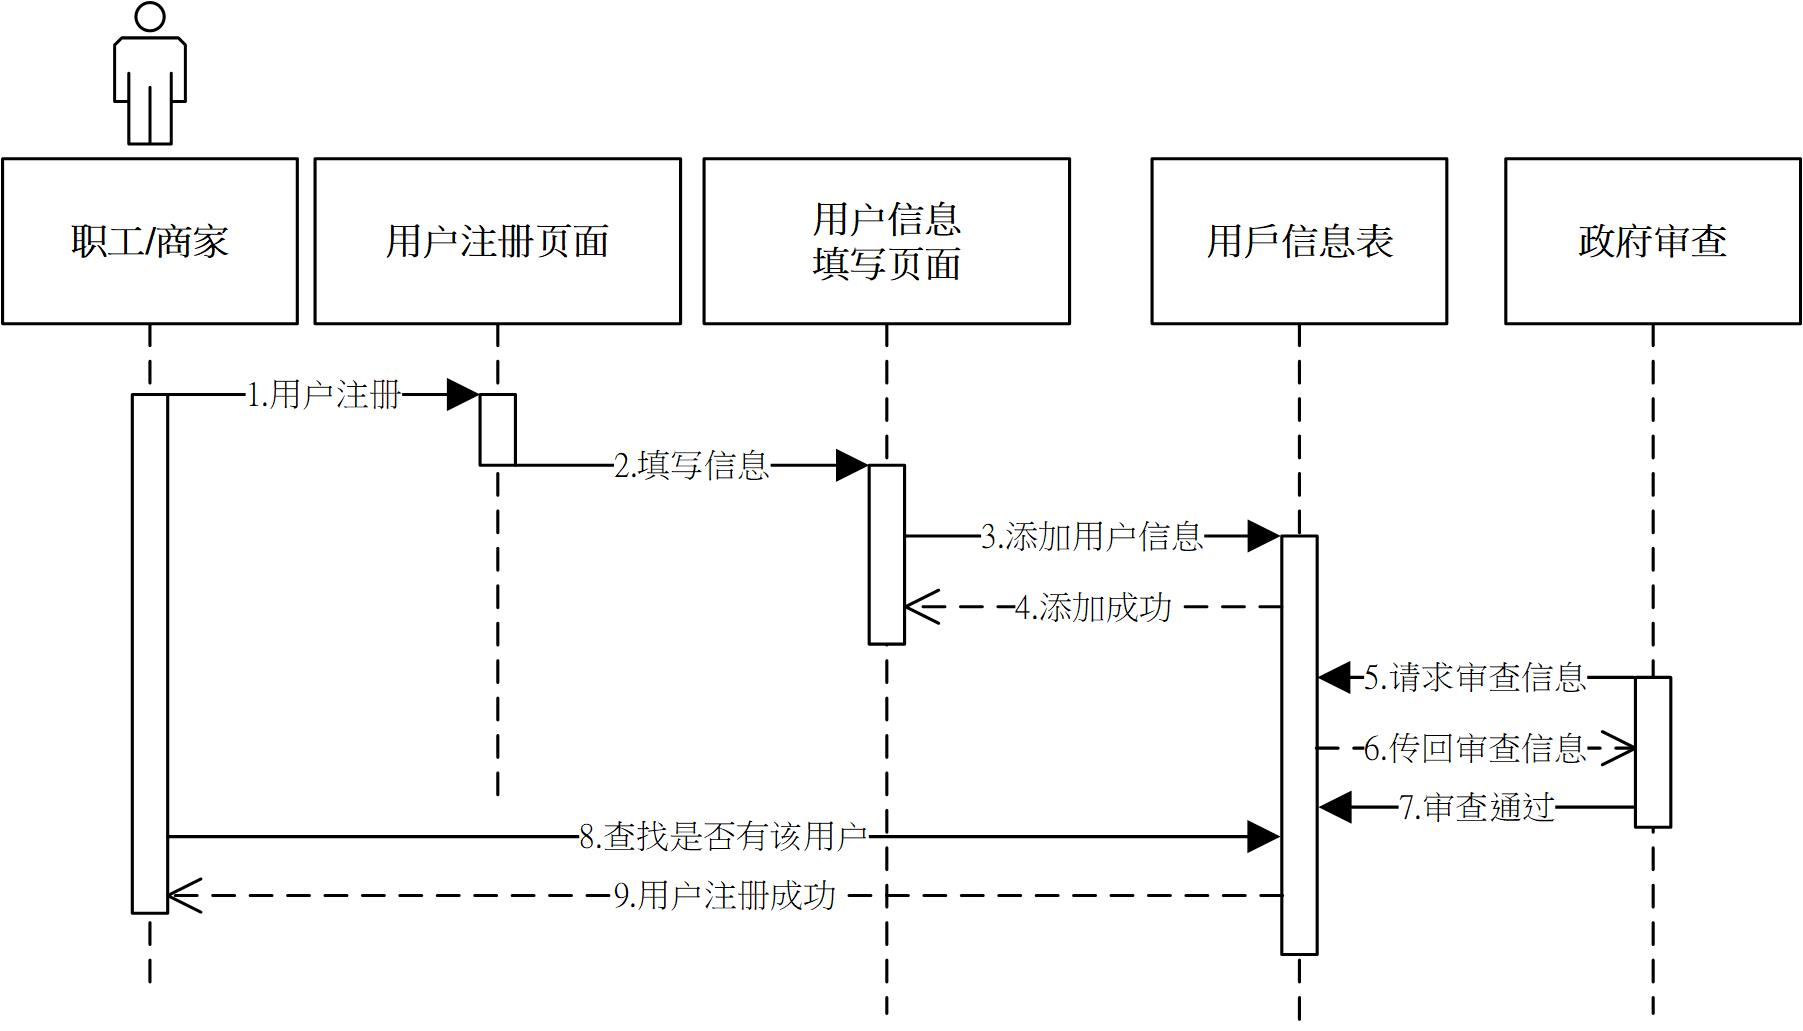
\includegraphics[width = 0.9\textwidth]{time1.jpg}
		\caption{職工與商家註冊時序圖}\label{time1}
	\end{figure}

	\begin{enumerate}
	\item 首先職工或是商家前往用戶註冊頁面。
	\item 前往用戶信息填寫頁面填寫用戶帳戶信息以及用戶密碼。
	\item 完成填寫後,為了提升用戶密碼信息安全,將用戶密碼以哈希算法計算後以密碼哈希值保存。將填寫完的帳號信息以及密碼哈希值提交到用戶信息表。
	\item 用戶信息表則傳回添加成功。屆時的用戶信息已經存儲到用戶信息表內但是尚未被激活,需要等待政府進行審查。
	\item 政府向用戶信息請求表拿取所有還未被激活的用戶信息。
	\item 數據庫中的用戶信息表傳回,政府請求的用戶信息清單。
	\item 政府進行用戶審查,在完成用戶審查後,則向用戶信息表內輸入審查通過。
	\item 此時,用戶再次訪問用戶信息表當中,用戶帳號是否已經激活成功。
	\item 用戶信息表回傳已經驗證通過。
	\end{enumerate}


\subsubsection{(二)商家產品管理模塊}
商家的運營需要管理本⾝所需販售的商品。在商家完成註冊⽤⼾帳號並且通過政府審核之後,便可檢視所有的產品,近⼀步可以透過產品管理模塊新增、修改以及刪除商家商品。圖\ref{c2}為商家產品管理類圖,其中StoreProductManagement 類中有四個⽅法需要實現,分別為顯⽰商家信息的showstoreinfo() ⽅法、顯⽰商家產品信息的showstoreproductinfo() ⽅法、顯⽰產品信息的showproductinfo() 以及修改商家產品信息的edit()⽅法。其中StoreProductCompare 類與EditStoreProduct 類需要向StoreProduct 請求商家產品信息,StoreProductCompare 類中的compare() ⽅法是向商家產品信息表取得與STORE\_ID 相符的所有相關商家產品。EditStoreProduct 類中的addstoreproduct() ⽅法、editstoreproduct() ⽅法、以及deletestoreproduct() ⽅法分別為新增、修改、以及刪除商家產品信息。StoreCompare 類中的compare() ⽅法是向Store 類請求與STORE\_ID 相符的商家信息。

	\begin{figure}[!htbp]
		\centering
		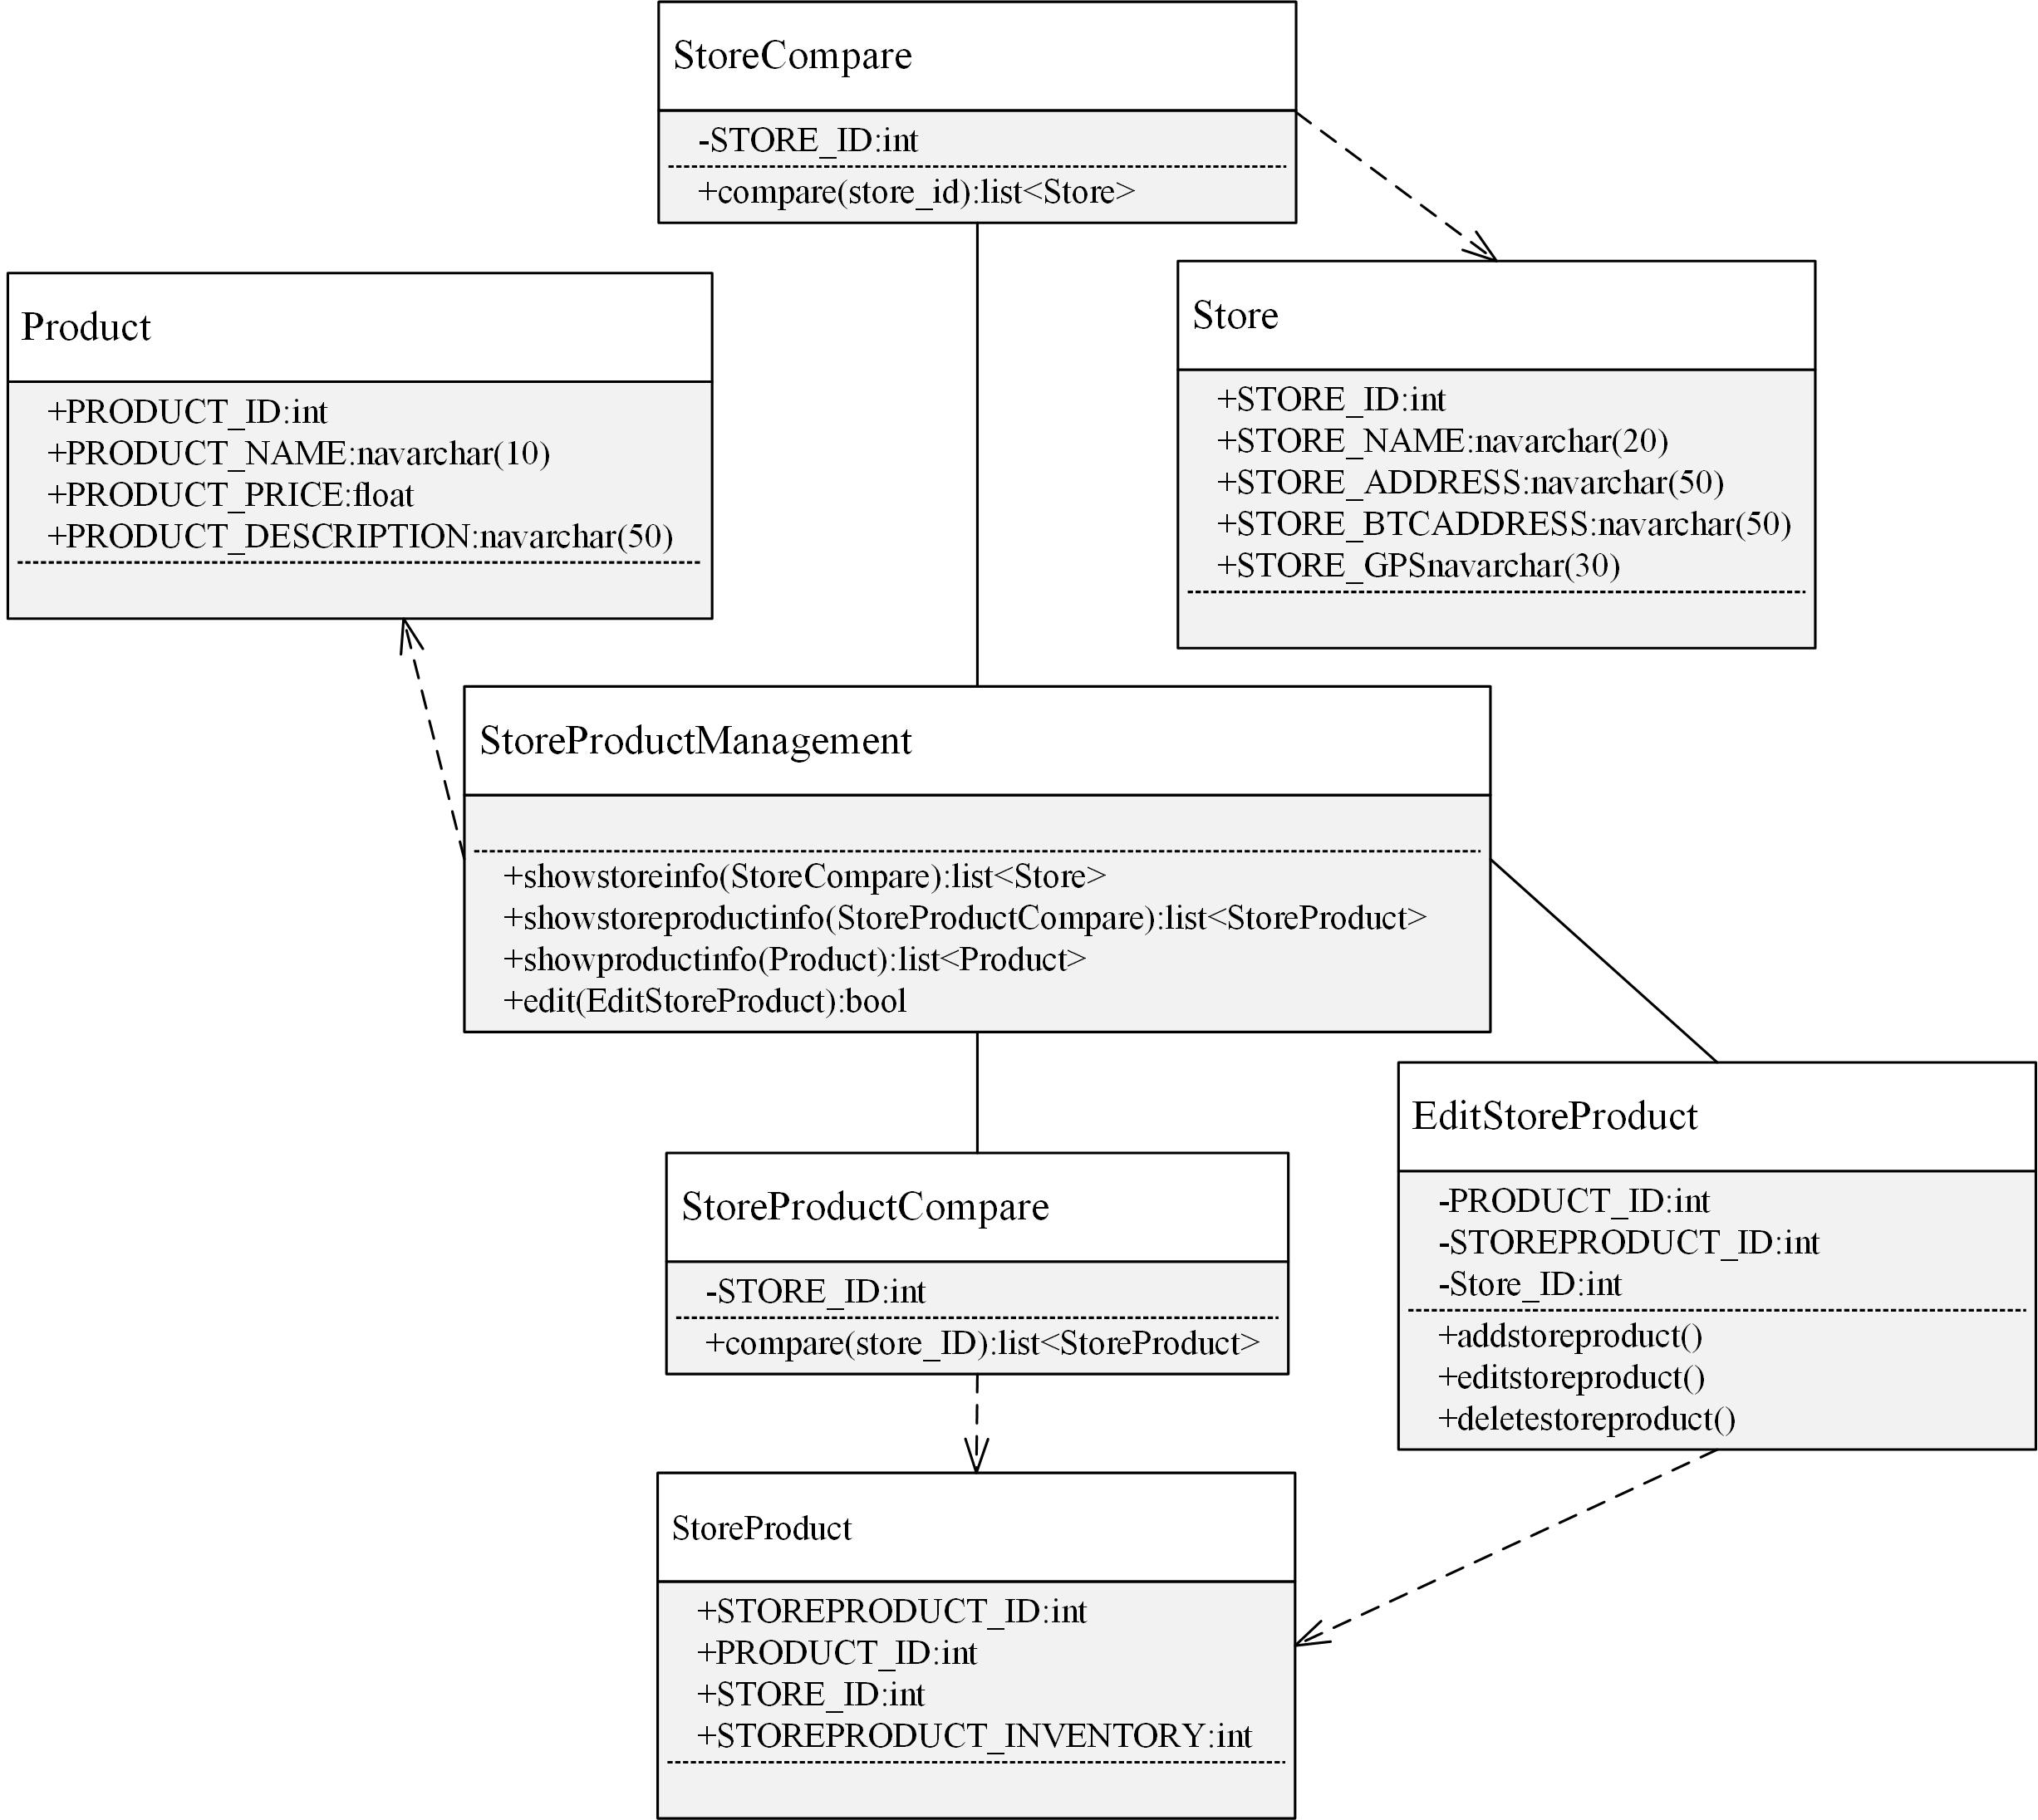
\includegraphics[width = 0.9\textwidth]{c2.jpg}
		\caption{商家產品管理類圖}\label{c2}
	\end{figure}

	圖\ref{time3}為商家產品管理時序圖,以下為流程說明:

	\begin{figure}[!htbp]
		\centering
		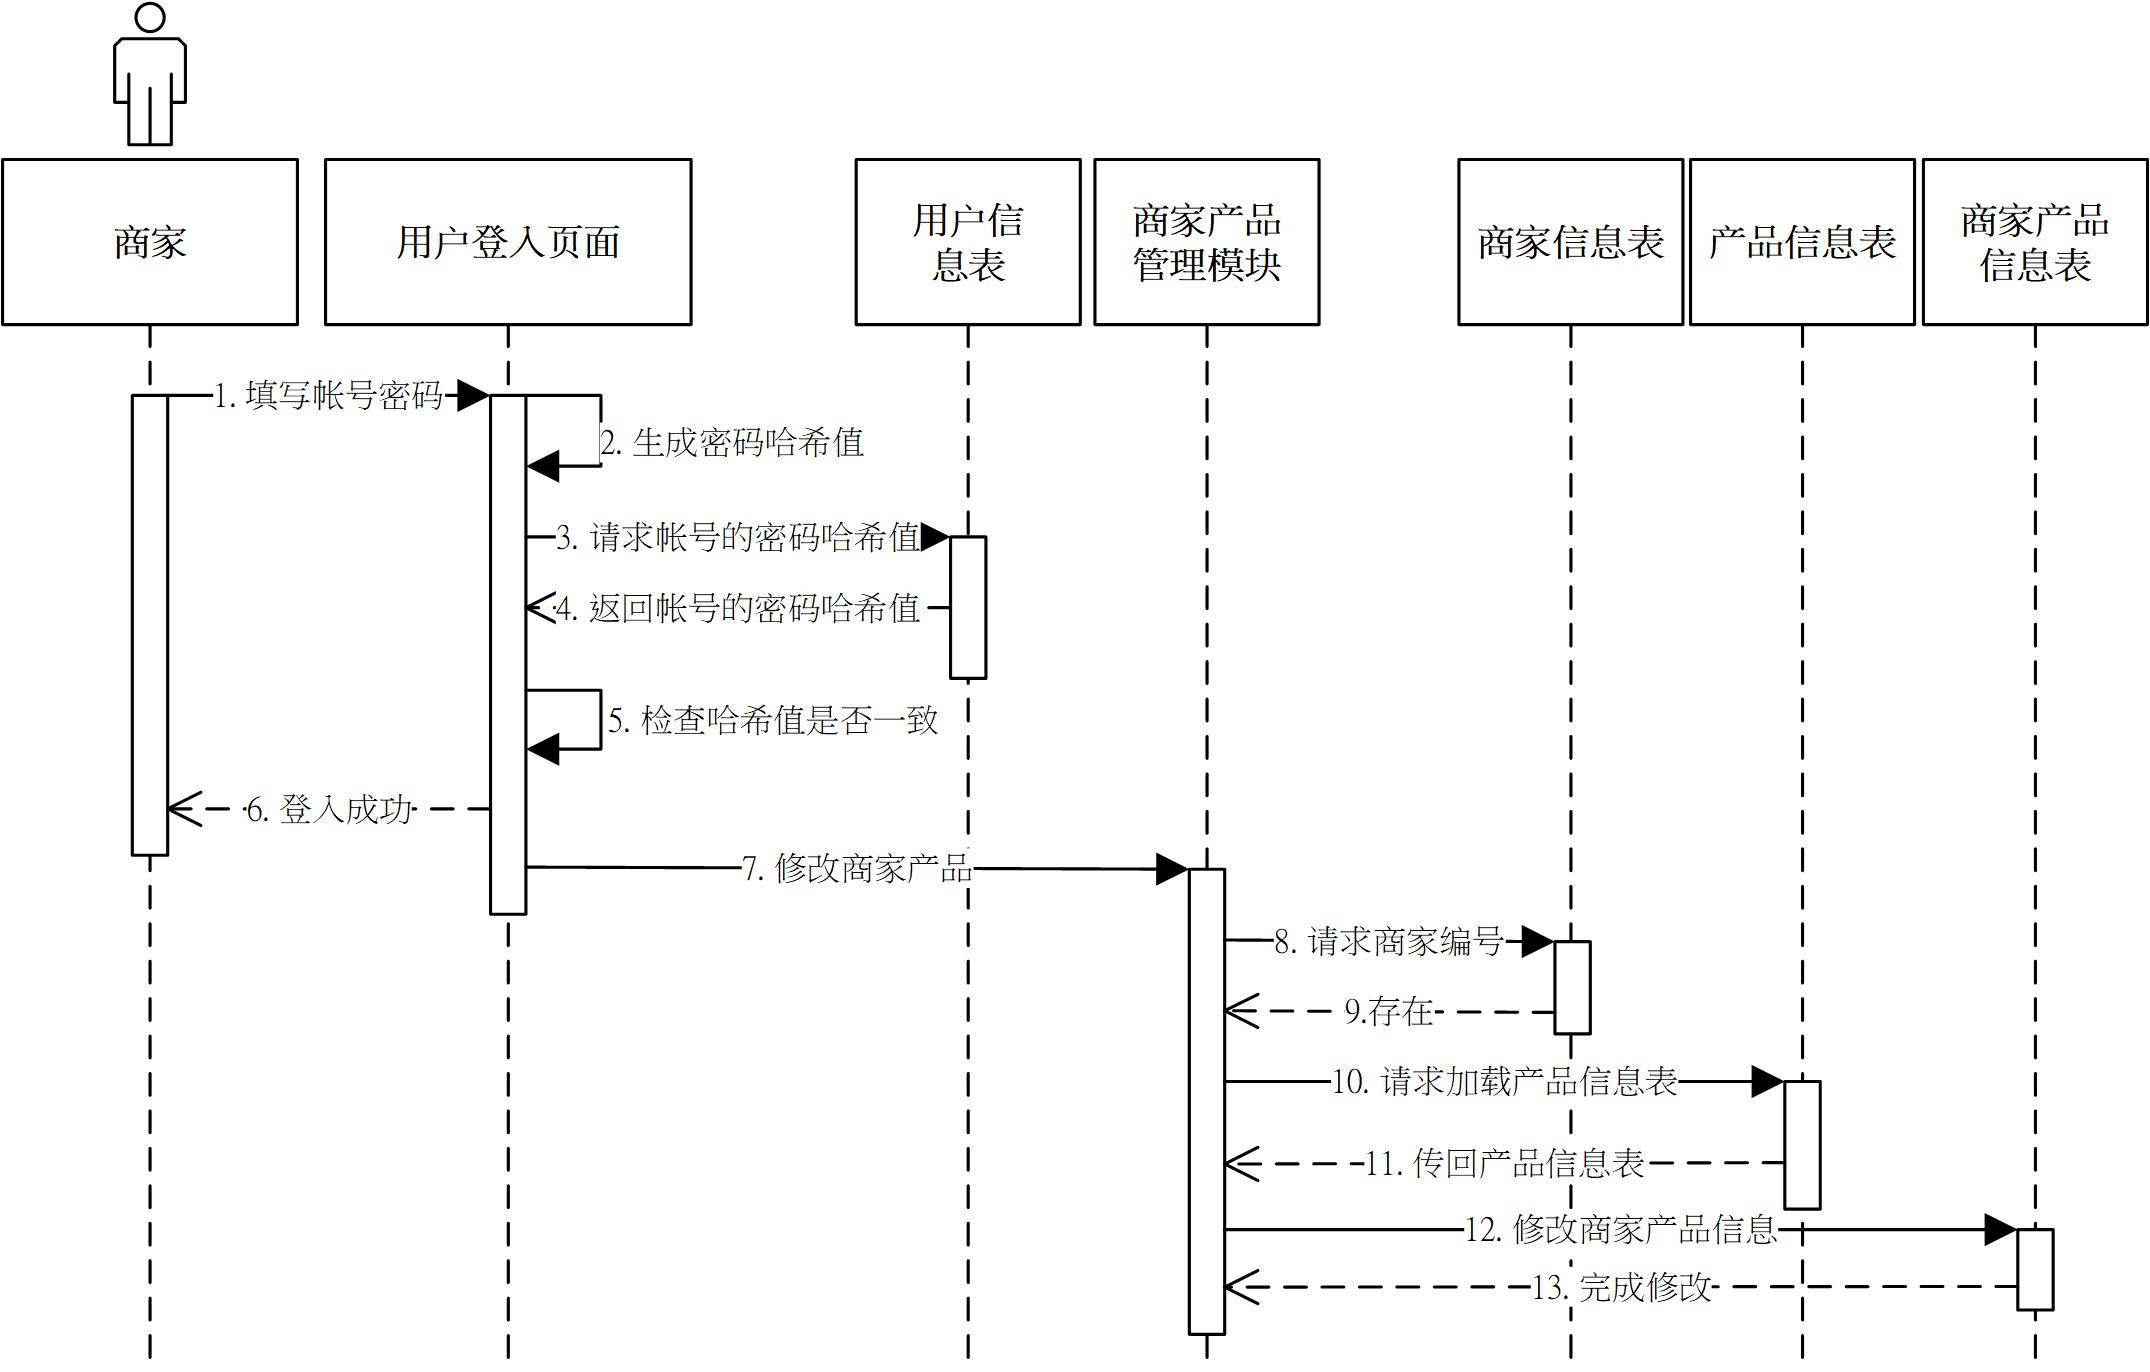
\includegraphics[width = 0.9\textwidth]{time3.jpg}
		\caption{商家產品管理時序圖}\label{time3}
	\end{figure}

	\begin{enumerate}
	\item 商家在完成用戶註冊後並完成政府的審核之後,便可填寫使用用戶與用戶密碼到登入頁面。
	\item 登入頁面會將用戶提交之密碼透過哈希算法生成密碼哈希值。
	\item 用戶登入頁面向用戶信息表詢問該用戶帳號的密碼哈希值。
	\item 用戶信息表將該帳戶的密碼哈希值傳回給用戶登入頁面保存。
	\item 用戶頁面將本地密碼哈希值和從數據庫信息表中請求保存的密碼哈希值進行比對是否相同。
	\item 倘若本地與數據庫中的哈希值一致,則為登入成功。
	\item 屆時可以進入商家產品管理模塊。
	\item 為確認欲修改的商家是否存在,所以向數據庫中的商家信息表請求該商家編號是否存在。
	\item 商家信息表返回存在的信息。
	\item 向數據庫中的產品信息表當中請求所有的產品信息。
	\item 產品信息表回傳所有的產品信息。
	\item 此時商家已經確認商家信息是否存在,且已經取得所有的產品信息。商家向商家產品信息表提交商家要增加的產品編號以及商家本身的商家編號,此時生成商家產品編號。
	\item 商家信息表在完成添加商家產品信息之後,傳回添加成功的信息到商家產品管理模塊。
	\end{enumerate}


\subsubsection{(三)職工管理模塊}
商家需要職⼯進⾏商家的運營。在商家⽤⼾完成政府審查之後,便可以進⼊職⼯管理模塊,透過提交⽤⼾編號以及商家編號新增、修改以及刪除職⼯信息。圖\ref{c1}為職⼯管理模塊類圖,StaffManagement 類當中有四種⽅法,前三種分別為顯⽰與該商家STORE\_ID 相符的完整信息showstore() ⽅法、顯⽰符合該商家STORE\_ID 職⼯信息的showstorestaff() ⽅法、顯⽰⽤⼾編號的showuser() ⽅法。而在第四種方法中,UserCompare 類需要向User 類提取⽤⼾相關信息實現查詢,StoreCompare 類需要向Store 類請求商家信相關信息,其中EditStoreStaff 類與StoreStaffCompare 類需要使⽤到Staff 類修改職⼯信息表的內容,EditStoreStaff 類中的addstaff()、editstaff() 以及deletestaff() ⽅法分別為新增、修改以及刪除職⼯,StoreStaffCompare 類中的compare ⽅法是取得符合STORE\_ID 的所有職⼯信息。

	\begin{figure}[!htbp]
		\centering
		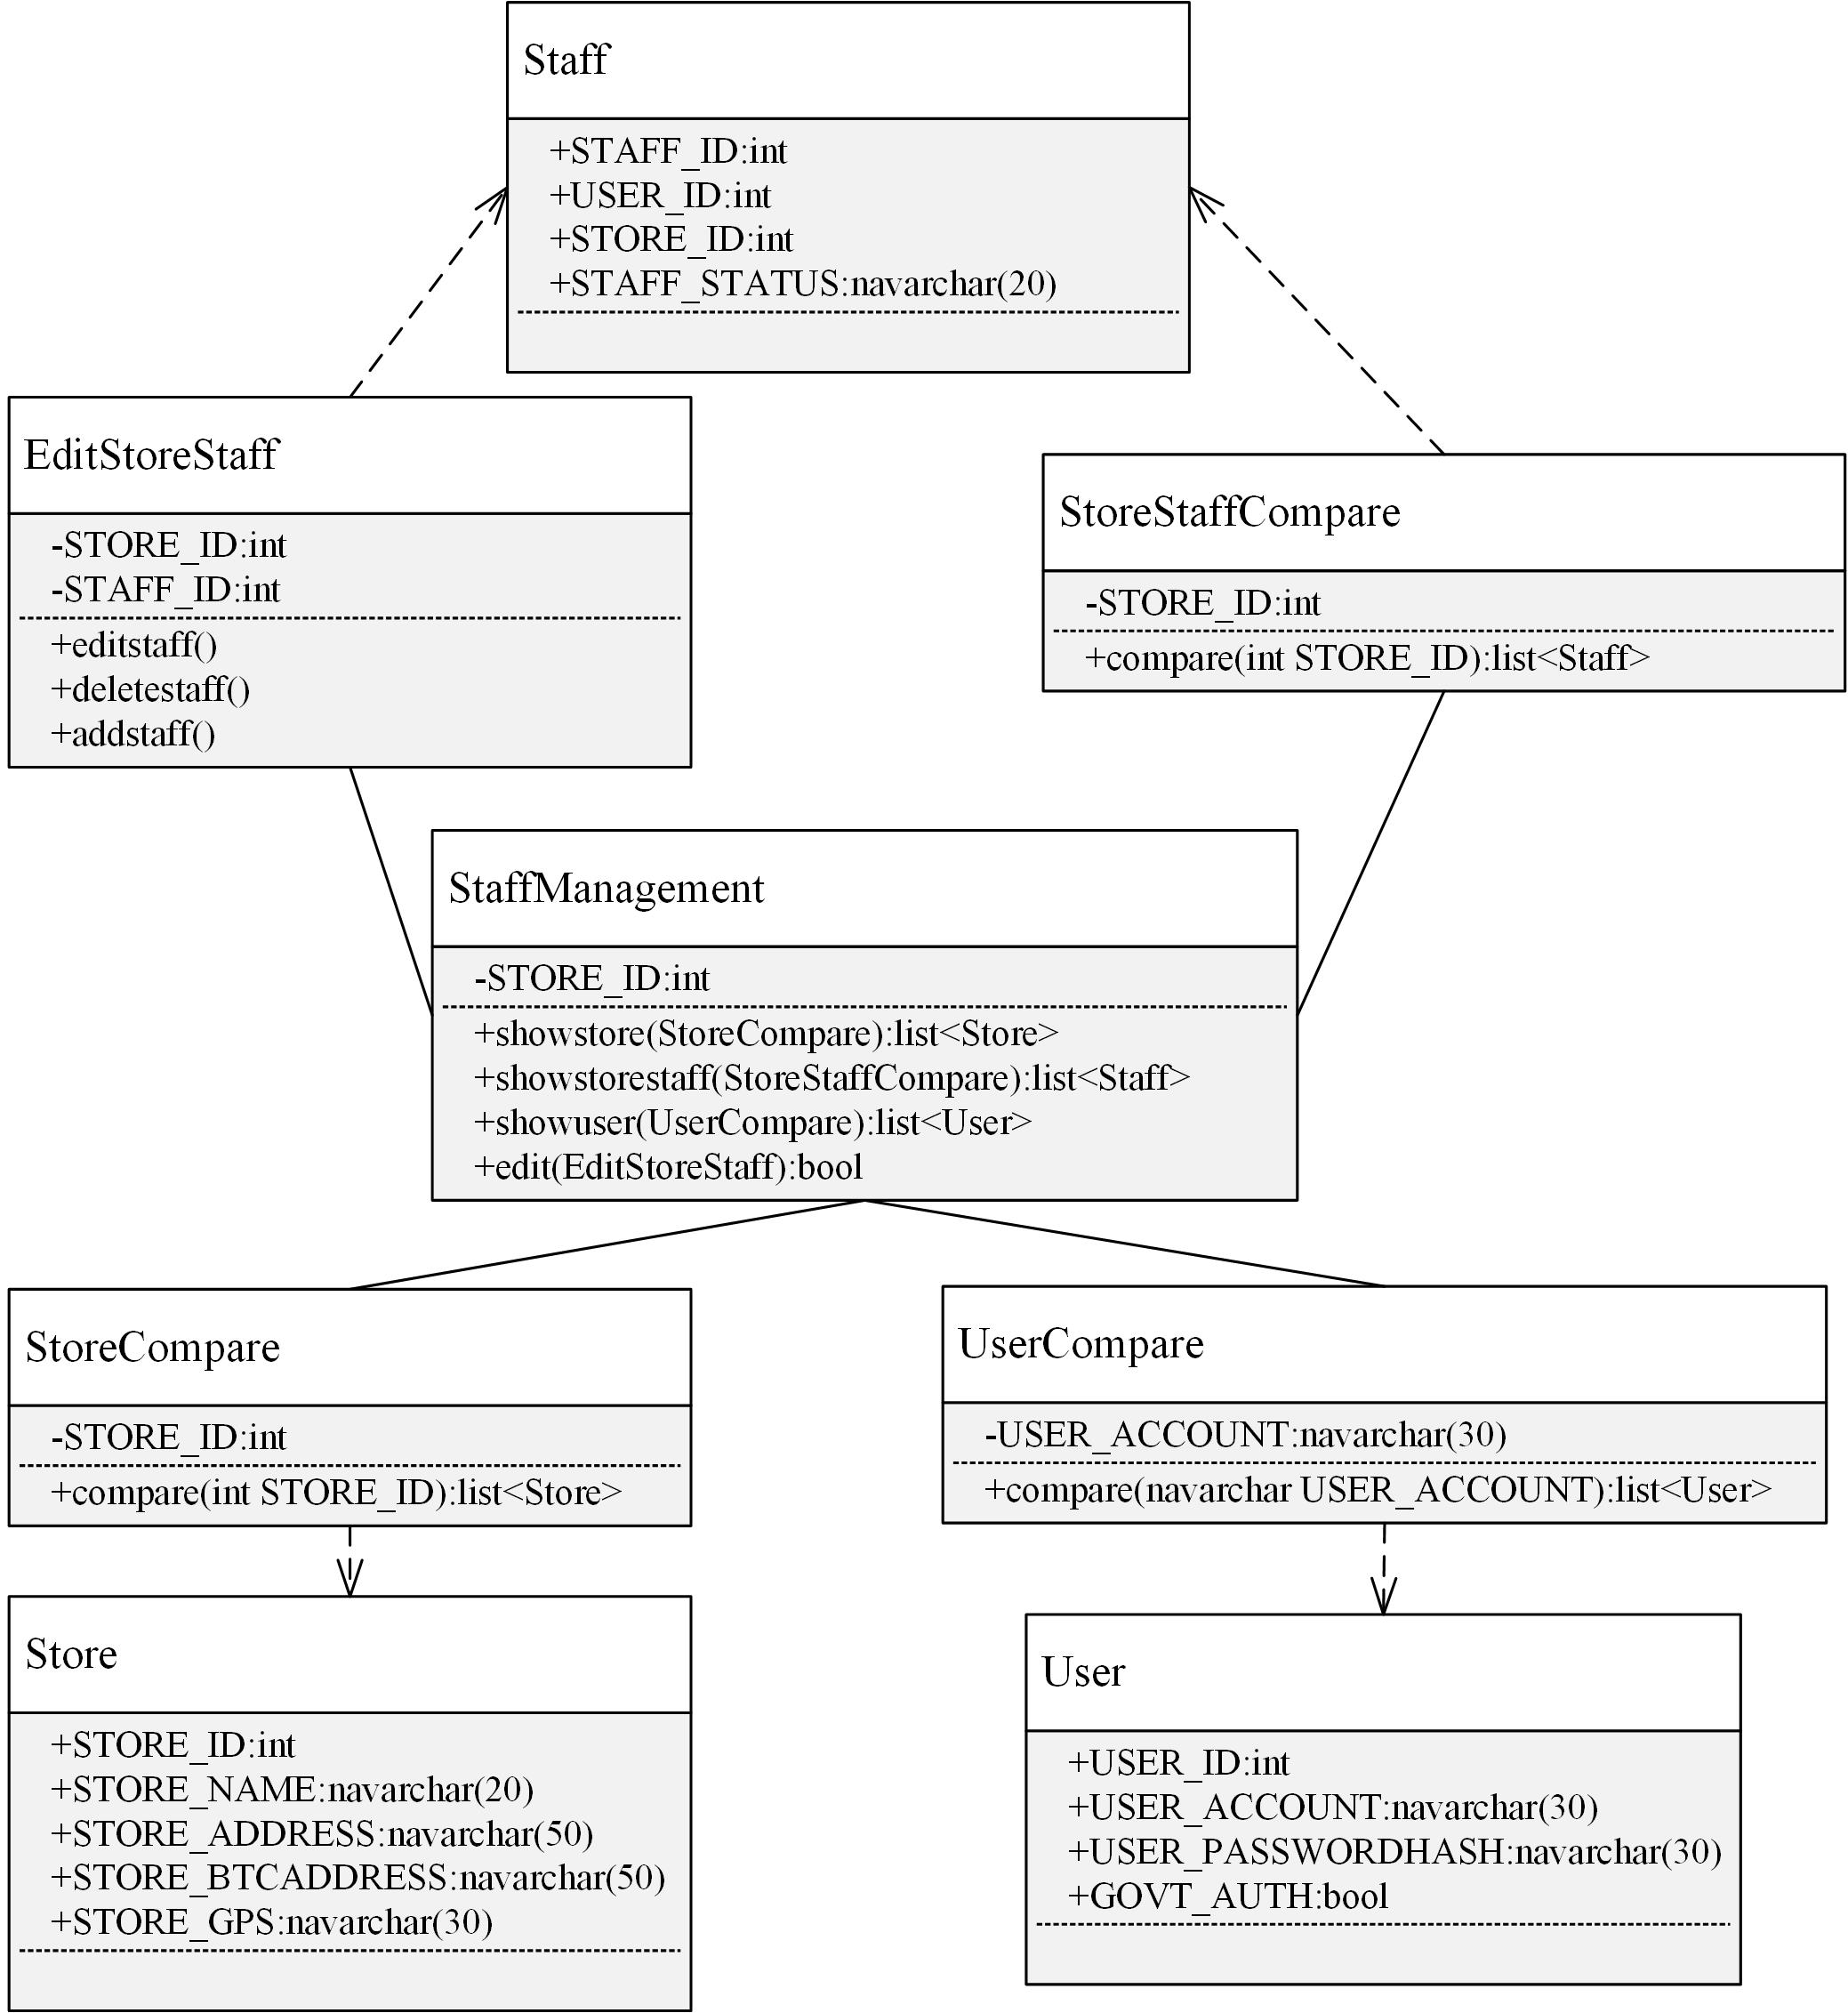
\includegraphics[width = 0.8\textwidth]{c1.jpg}
		\caption{職工管理模塊類圖}\label{c1}
	\end{figure}

	

	圖\ref{time2}為商家職工管理時序圖,以下為流程說明:

	\begin{figure}[!htbp]
		\centering
		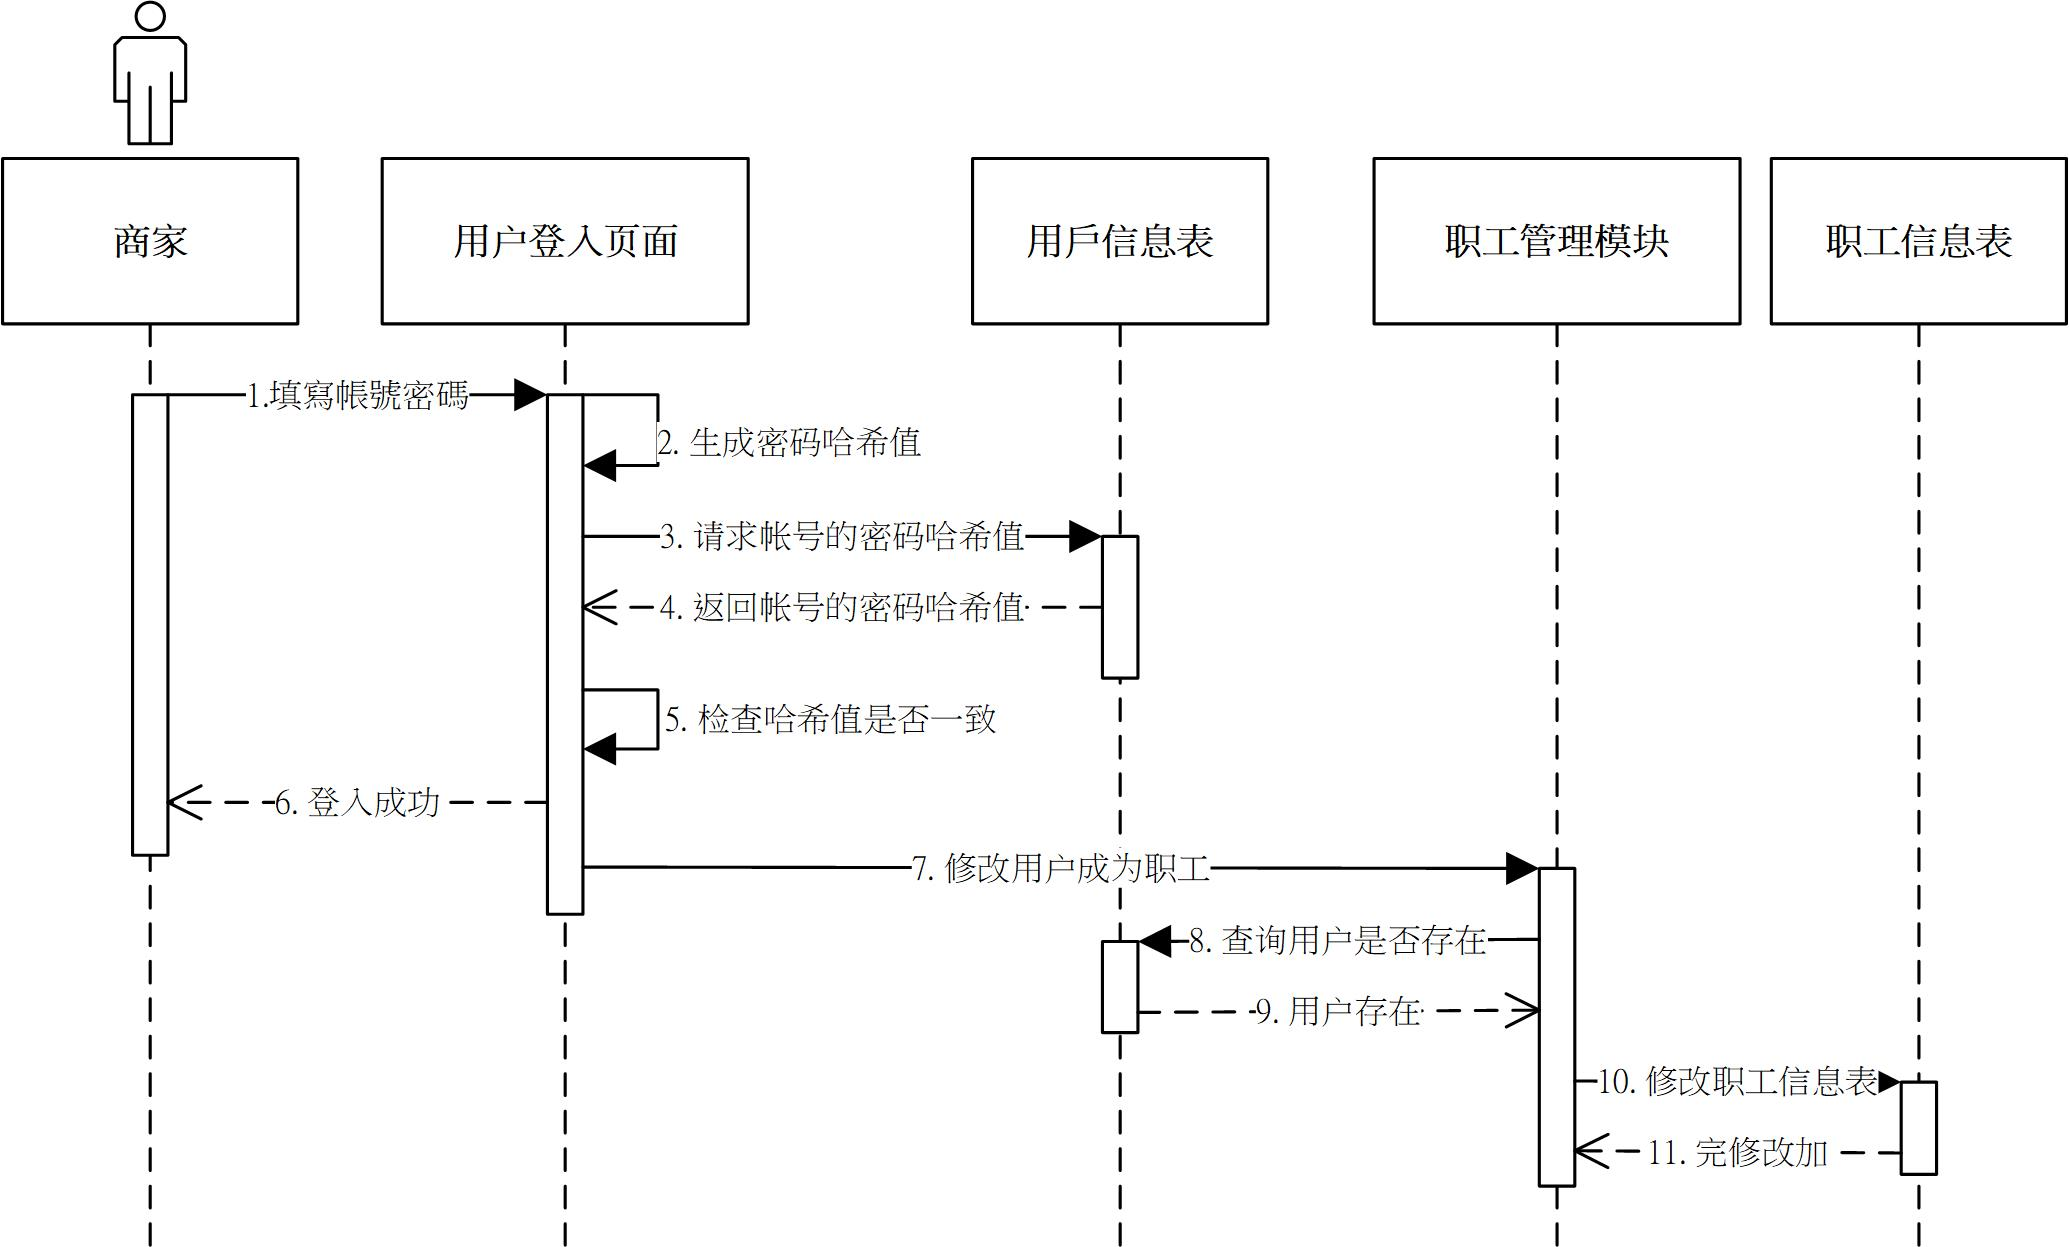
\includegraphics[width = 0.9\textwidth]{time2.jpg}
		\caption{商家職工管理時序圖}\label{time2}
	\end{figure}

	\begin{enumerate}
	\item 商家前往用戶登入頁面輸入用戶帳號密碼。
	\item 用戶登入頁面自動使用哈希算法將用戶密碼轉換成密碼哈希值。
	\item 用戶登入頁面向數據庫中的用戶信息表請求該用戶帳號的密碼哈希值。
	\item 數據庫用戶信息表回傳用戶密碼哈希值。
	\item 用戶登入頁面比對本地端的用戶密碼哈希值與數據庫中的密碼哈希值是否一致。
	\item 倘若數據庫中的密碼哈希值與用戶登入頁面生成的密碼哈希值一致,則登入成功。
	\item 商家提交商家編號以及欲添加的用戶編號。
	\item 職工管理模塊向用戶信息表查詢該用戶是否存在。
	\item 用戶信息表傳回用戶存在信息。
	\item 職工管理模塊向數據庫中的職工信息表提交用戶編號、商家編號以及職工編號修改職工信息。
	\item 職工信息表傳回修改完成。
	\end{enumerate}

\subsubsection{(四)商家交易管理模塊}
在⽤⼾完成註冊後且在商家將該⽤⼾加⼊成為公司職⼯後,該職⼯可以透過⽤⼾帳號進⼊到商家交易管理模塊,該模塊為移動裝置的應⽤程序。在進⼊到本模塊後會⾃動加載商家商品、商家信息以及職⼯信息,製成⼀個基於區塊鏈加密貨幣的移動收銀機,可以掃描帶有RFID 標籤的商家產品,創建交易後等待⽤⼾交易管理模塊讀取以及驗證交易是否完成的信息。图5.8為商家交易管理模塊類圖,在StoreTransactionManagement 類當中有五個⽅法,分別為顯⽰所有的商家產品信息的showstoreproduct() ⽅法、顯⽰職⼯信息的showstorestaff()⽅法、顯⽰商家信息的showstore() ⽅法、檢查交易是否完成的check() ⽅法以及透過NFC 傳輸協議傳輸信息的nfc() ⽅法。StoreCompare 類中的compare() ⽅法是向Store類取得與STORE\_ID 相符的商家信息,StoreProductCompare 類中的compare() ⽅法是向StoreProduct 類請求與STORE\_ID 相符的所有商家產品信息。StoreStaffCompare 類中的compare() ⽅法是向Staff 類中請與USER\_ID 相符的職⼯信息。在NFCMessage 類中有兩個⽅法,receivenfcmessage() ⽅法使得商家可以快速的掃描商品的RFID 標籤,sendnfcmessage() ⽅法使得職⼯在創建完交易清單後可以將交易信息傳送給顧客。CheckTx 類中有兩個⽅法,分別為取得於Tx 類中交易信息的compare() ⽅法,以及getcheck()⽅法是檢查該筆交易的CHECK 值是否已經在Tx 類中被修改為"1",倘若被修改為"1"則表示該筆交易已經被寫⼊區塊鏈中。在本模塊要做到驗證⽐特幣交易是否已經被存儲在⽐特幣區塊鏈當中,必須使⽤BlockchainExplore 類中的getblockchain() ⽅法取得所有區塊鏈相關的信息,再透過getbitcointx() ⽅法取得該筆⽐特幣交易的狀態以及詳細信息。Tx 類中可以調⽤txcheck() ⽅法對BlockchainExplore 類檢查該筆交易是否已經進⼊了區塊鏈,如果已經進⼊區塊鏈,則將相關的交易信息的CHECK 值修改為"1"。值得⼀提的是,在此將CHECK 值修改為"1" 的標準,為該筆交易進⼊區塊鏈的時間。由於⽐特幣區塊鏈的⽣成速度平均為每⼗分鐘⼀塊,這將使得交易確認速度不夠即時。


	\begin{figure}[!htbp]
		\centering
		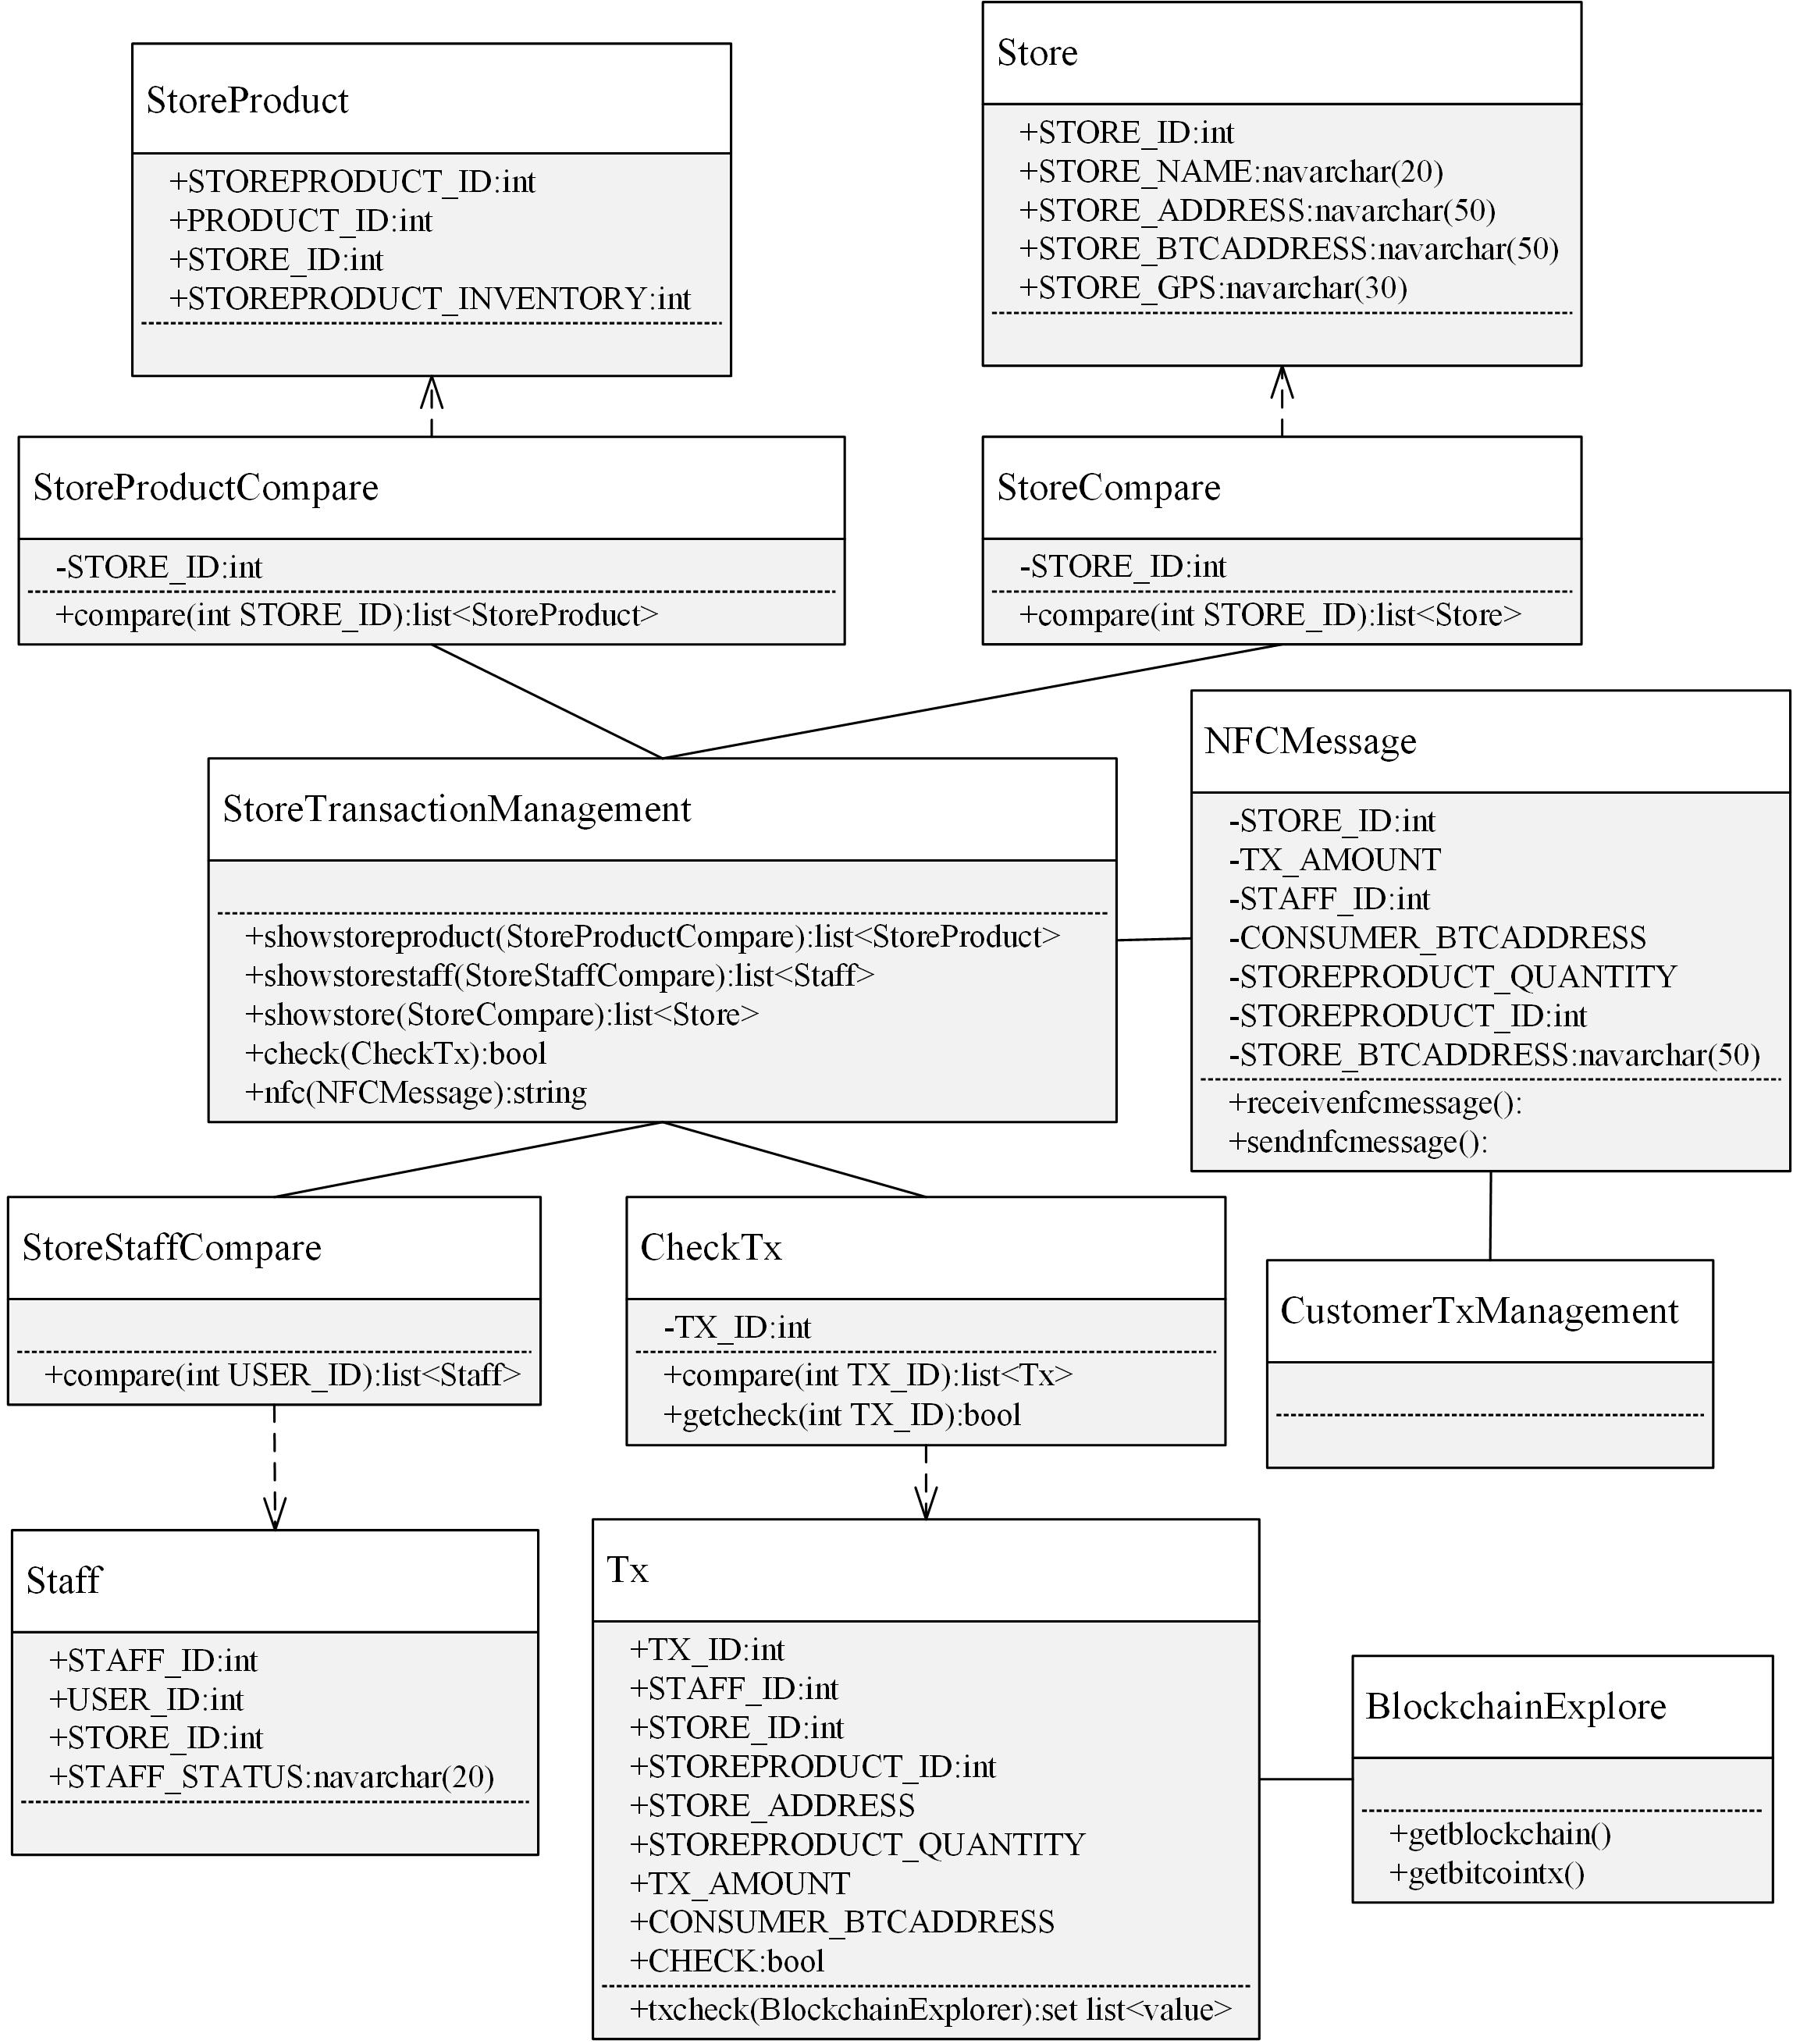
\includegraphics[width = 0.9\textwidth]{c5.jpg}
		\caption{商家交易管理模塊類圖}\label{c5}
	\end{figure}


圖\ref{time4}為商家交易管理時序圖,以下為流程說明:

	\begin{figure}[!htbp]
		\centering
		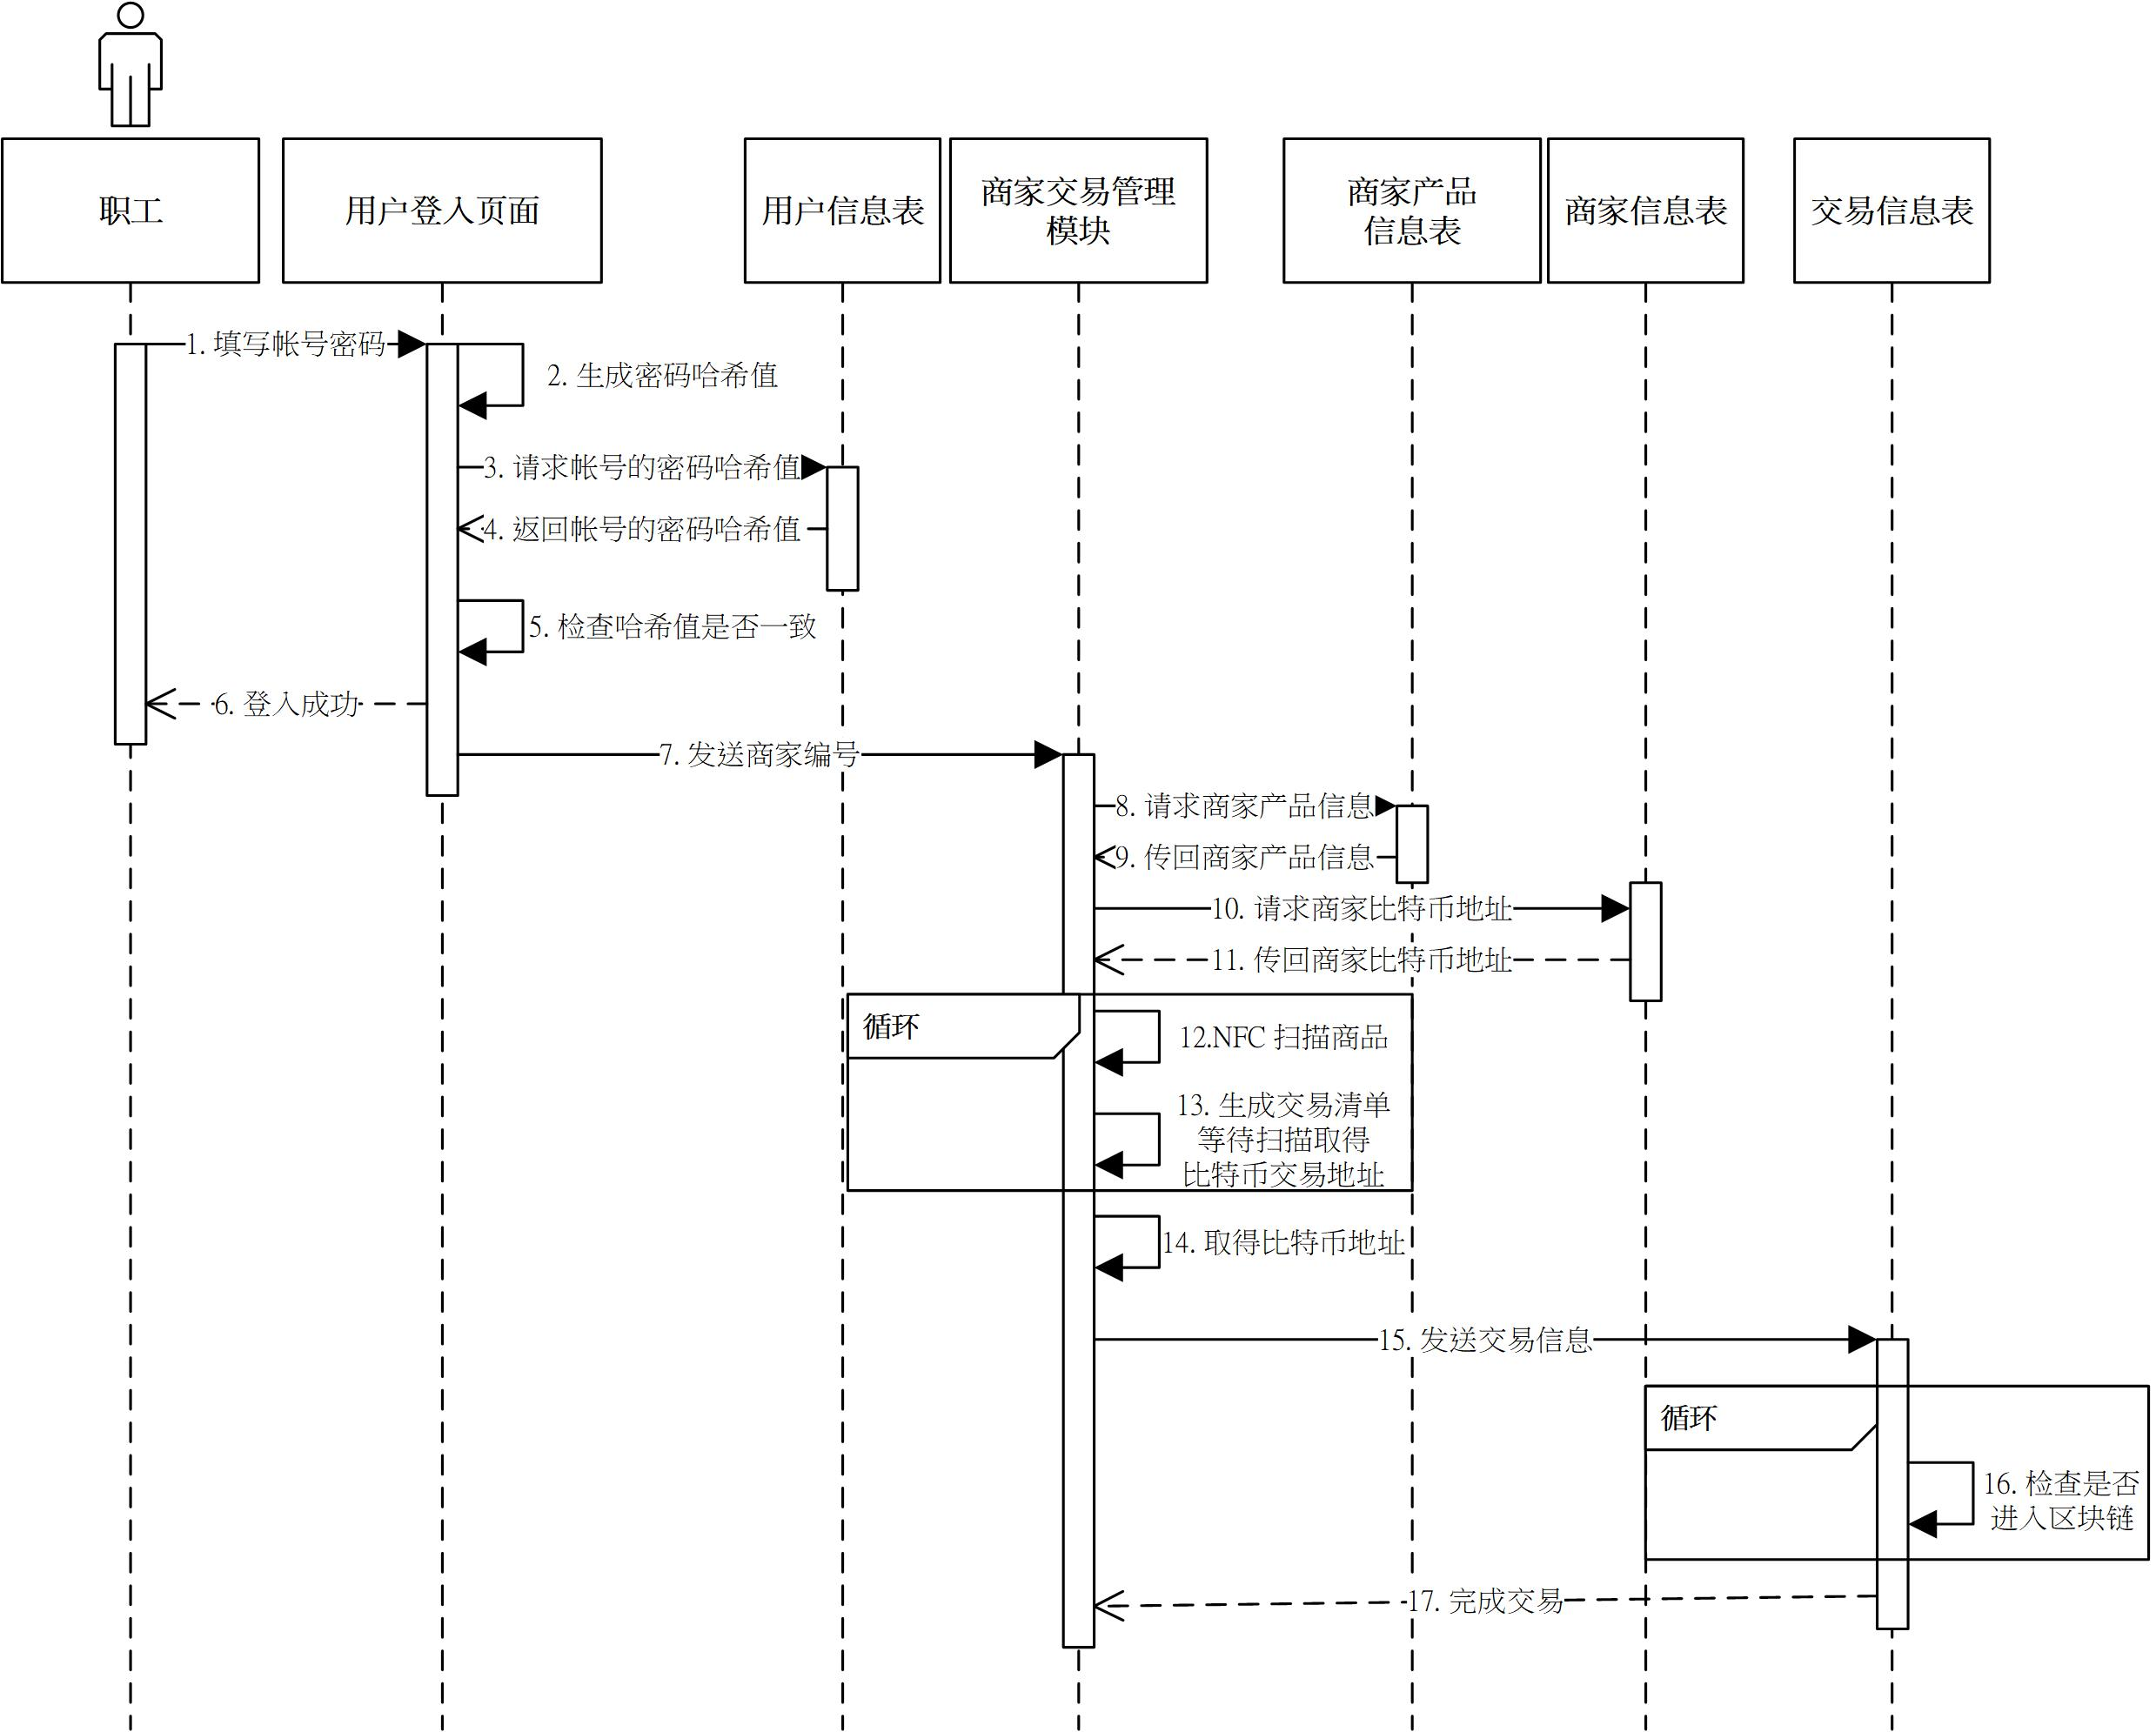
\includegraphics[width = 1\textwidth]{time4.jpg}
		\caption{商家交易管理時序圖}\label{time4}
	\end{figure}

	\begin{enumerate}
	\item 首先職工填寫用戶的帳號密碼到用戶登入頁面。
	\item 用戶登入頁面模塊將用戶填寫的密碼透過哈希算法生成本地端的用戶密碼哈希值。
	\item 將用戶填寫的帳號發送到用戶信息表請求遠端的用戶密碼哈希值以及商家編號。
	\item 用戶信息表傳回遠端的用戶密碼哈希值。
	\item 用戶登入頁面模塊進行本地用戶密碼哈希值和遠端用戶密碼哈希值比對是否一樣。
	\item 倘若一致則登入成功。
	\item 此時用戶登入頁面向商家交易管理模塊發送商家編號的信息,商家交易管理模塊將信息保存。
	\item 商家交易管理模塊向商家產品信息表請求與商家編號相關的所有商家產品信息。
	\item 商家產品信息表傳回所有與商家相關的商家產品信息至商家交易管理模塊。
	\item 商家交易管理模塊向商家信息表請求商家比特幣地址信息。
	\item 商家信息表將商家比特幣地址信息傳回到商家交易管理模塊。
	\item 商家產品信息表將所有與商家編號有關的商家產品信息傳回到商家交易管理模塊,此時商家交易管理模塊已經有完整的商家產品信息以及商家信息。將帶有RFID標籤的商品透過NFC線圈進行感測對應到相關的商家產品信息。
	\item 將產品信息建立交易清單顯示在移動裝置的屏幕上,等待顧客的手持裝置進行感應,感應的同時會將交易清單以及商家比特幣地址傳送到顧客交易管理模塊。

	\item 在感應的同時顧客交易管理模塊會將比特幣錢包模塊中的比特幣地址提交給商家交易管理模塊。
	\item 商家交易管理模塊發送信息至交易信息表查找該筆交易信息。
	\item 交易信息表不斷的向區塊鏈檢視器查找該筆比特幣交易是否已經被寫入比特幣區塊鏈內,倘若寫入區塊鏈則將交易信息的CHECK信息由"0"改為"1"。
	\item 交易信息表傳回該筆交易的CHECK已經為"1"則完成交易
	
	\end{enumerate}

	在比特幣系統中,使得一筆比特幣交易得到比特幣網路的認可,需要等待六個區塊的交易驗證,相當於需要費時60分鐘的時間等待一個交易的完成,這使得比特幣交易在商家進行小額交易造成很大的不便,因此為了在BRTMS中改善此問題,便導入了基於Green Address錢包的多重簽章算法,使得交易時間可以從60分鐘的等待時間,縮短為一秒鐘左右。圖\ref{c7}為商家Government Green Address交易管理模塊類圖,在此模塊類圖中針對Tx類中添加ggatxcheck()方法,使得商家交易管理模塊可以支持Government Green Address地址格式的辨別,當檢測到為Government Green Address地址格式,將交易信息中的CHECK欄位修改為"1",這使得比特幣交易信息可以在平均一秒鐘的時間得到交易確認,ggatxcheck()方法需要調用BlockchainExplore類中的getblockchain()取得比特幣區塊鏈的信息以及getbitcointx()方法得到比特幣交易信息。在GovernmentGreenaddressCheckTx類中提供compare()方法可以針對Government Green Address地址向Tx類查詢相關信息以及ggatxcheck()方法檢測該筆交易是否存儲於交易信息中的CHECK值已經被修改為"1"。

	

	\begin{figure}[!htbp]
		\centering
		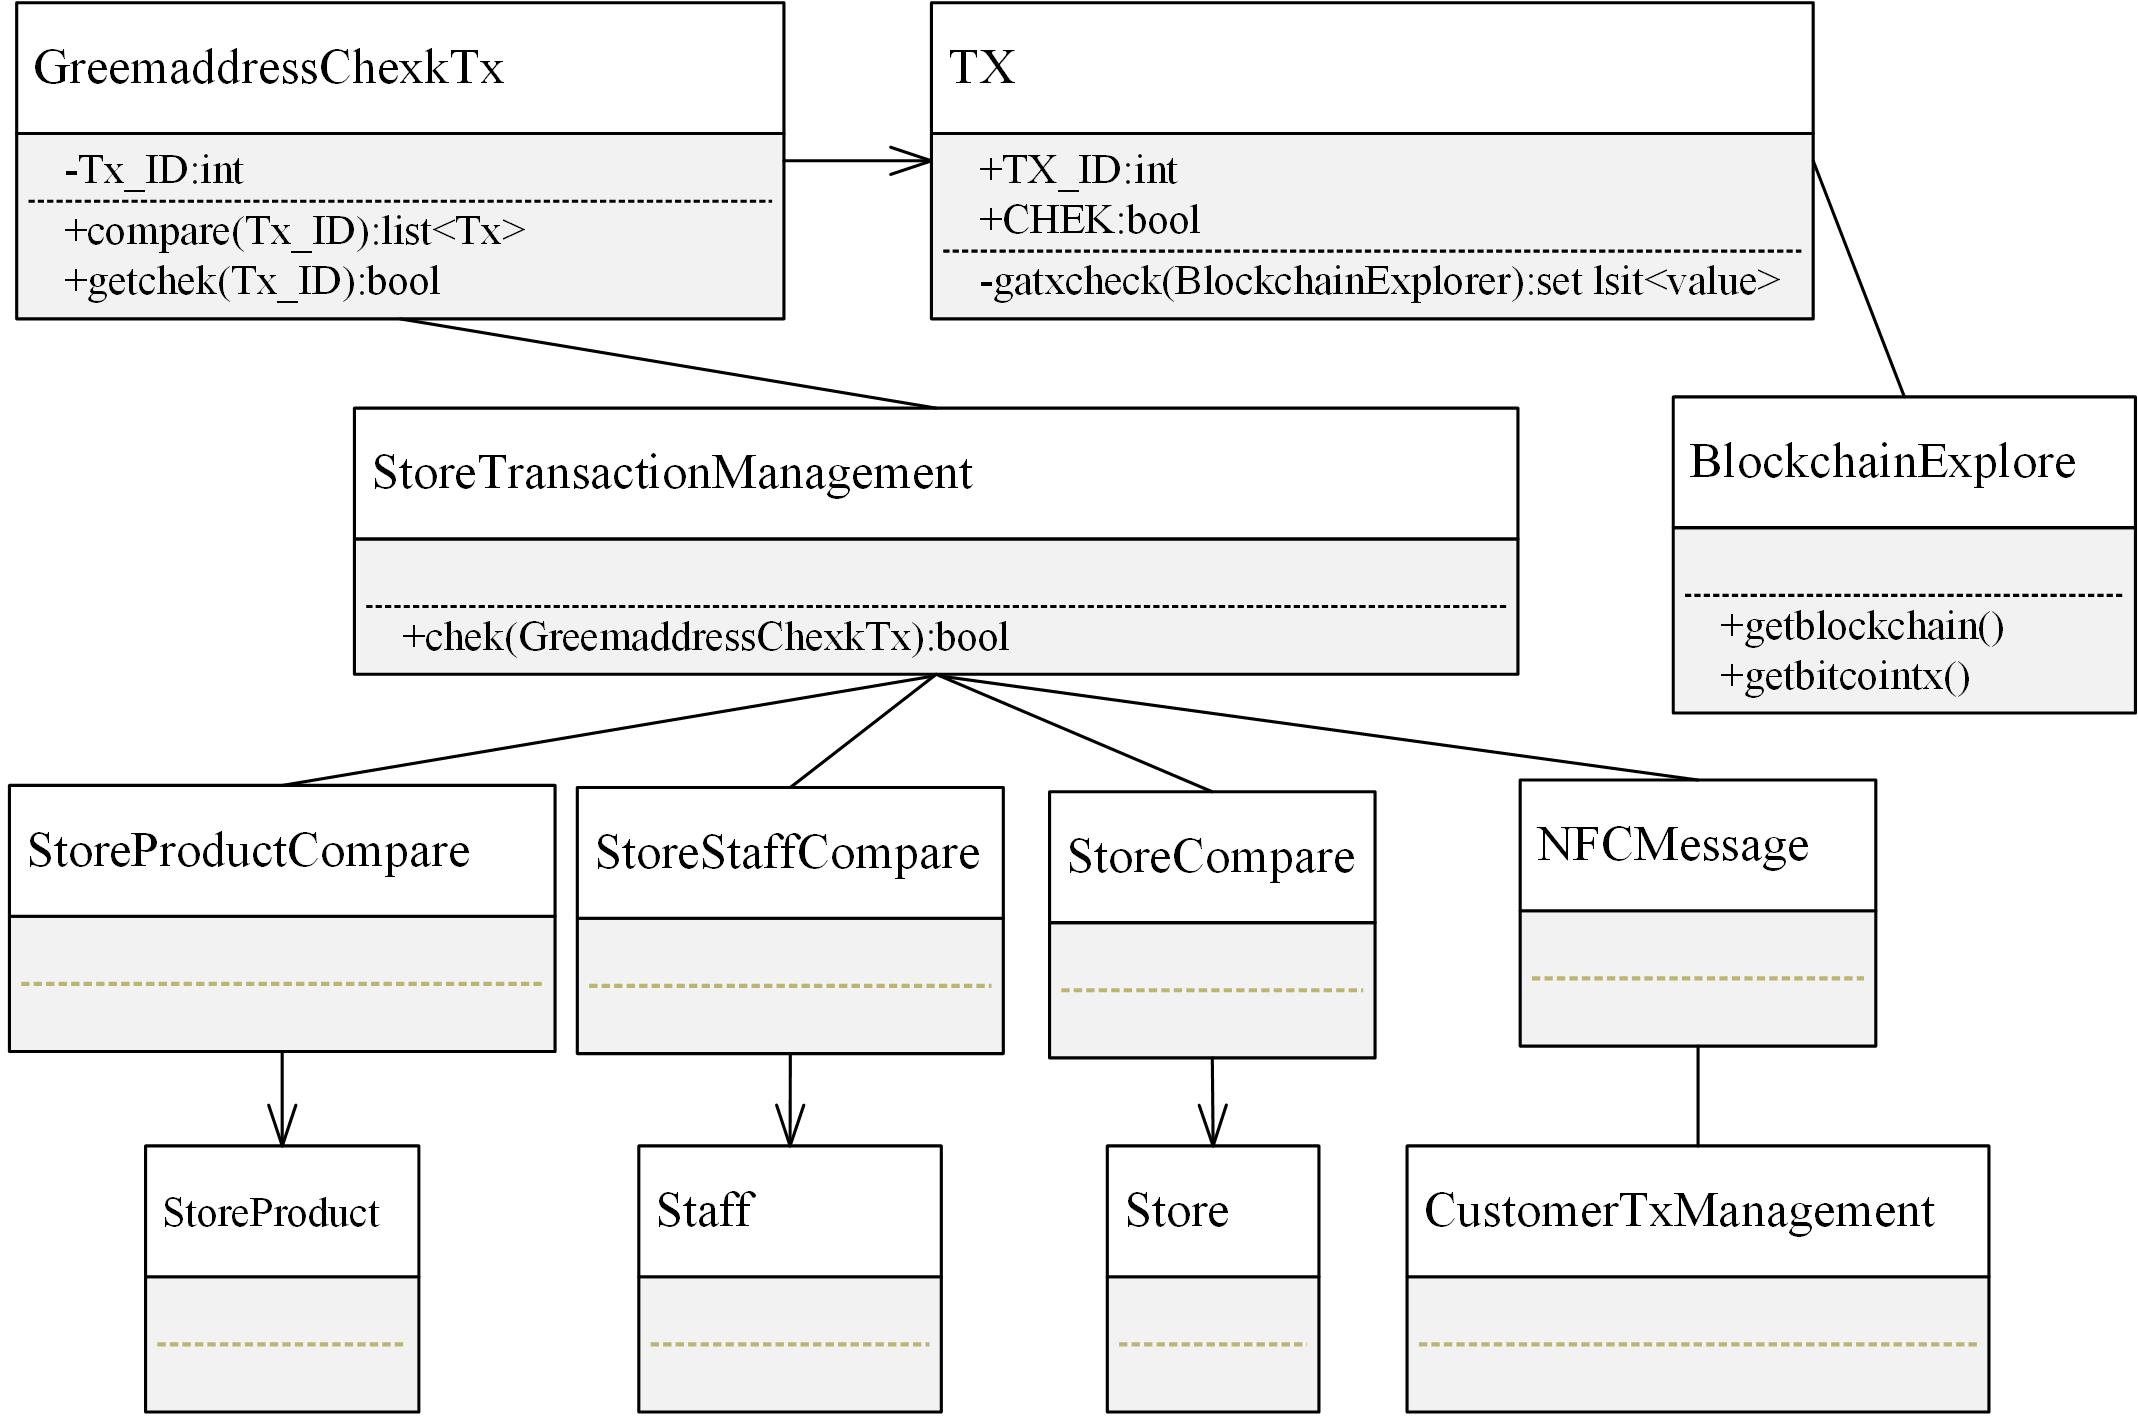
\includegraphics[width = 0.7\textwidth]{c7.jpg}
		\caption{商家Government Green Address交易管理模塊類圖}\label{c7}
	\end{figure}



\subsubsection{(五)顧客交易管理模塊}
在本系統中顧客需要在手持移動端安裝手機程序包括顧客交易管理模塊,使得顧客移動裝置可以支持比特幣支付、查詢過去的交易信息、以NFC通信協議接收商家交易管理模塊創建的交易信息以及詳細的商家商品信息。圖\ref{c4}為顧客交易管理模塊類圖,在CustomerTxManagement 類中包括六個⽅法,分別為顯⽰所有該⽤⼾擁有⽐特幣交易信息相關的交易明細的showtx() ⽅法、取得交易信息後取得相對應的商家產品信息的showstoreproduct() ⽅法、檢查於交易信息表中的交易信息CHECK 欄位的值是否已經被填⼊"1" 的check() ⽅法、發送詳細的交易信息⾄交易信息表保存的sendtx2table()⽅法、透過NFC 協議接收於StoreTransactionManagement 類所創建的交易信息以及發送⽤⼾⽐特幣地址的nfc() ⽅法,最後是控制⽐特幣錢包的bitcoinpayment() ⽅法。CheckTx類中的getcheck() ⽅法可以向Tx 類詢問該筆交易是否已經得到認證,TxCompare 類中的compare() ⽅法提供⽤⼾向交易信息表查找與⽤⼾交易信息相關的交易,TransferTx類中的sendtx() ⽅法是將顧客完成交易的交易信息提交到交易信息表,BitcoinPay 類使⽤pay() ⽅法⽀付⽐特幣,NFCMessage 類中的receivenfcmessage() 和sendnfcmessage()分別為透過NFC 協議發送以及接收交易信息和顧客⽐特幣地址。StoreProductCompare類則是向StoreProduct 類請求顧客移動裝置中所有交易信息中相關的商家商品。

	\begin{figure}[!htbp]
		\centering
		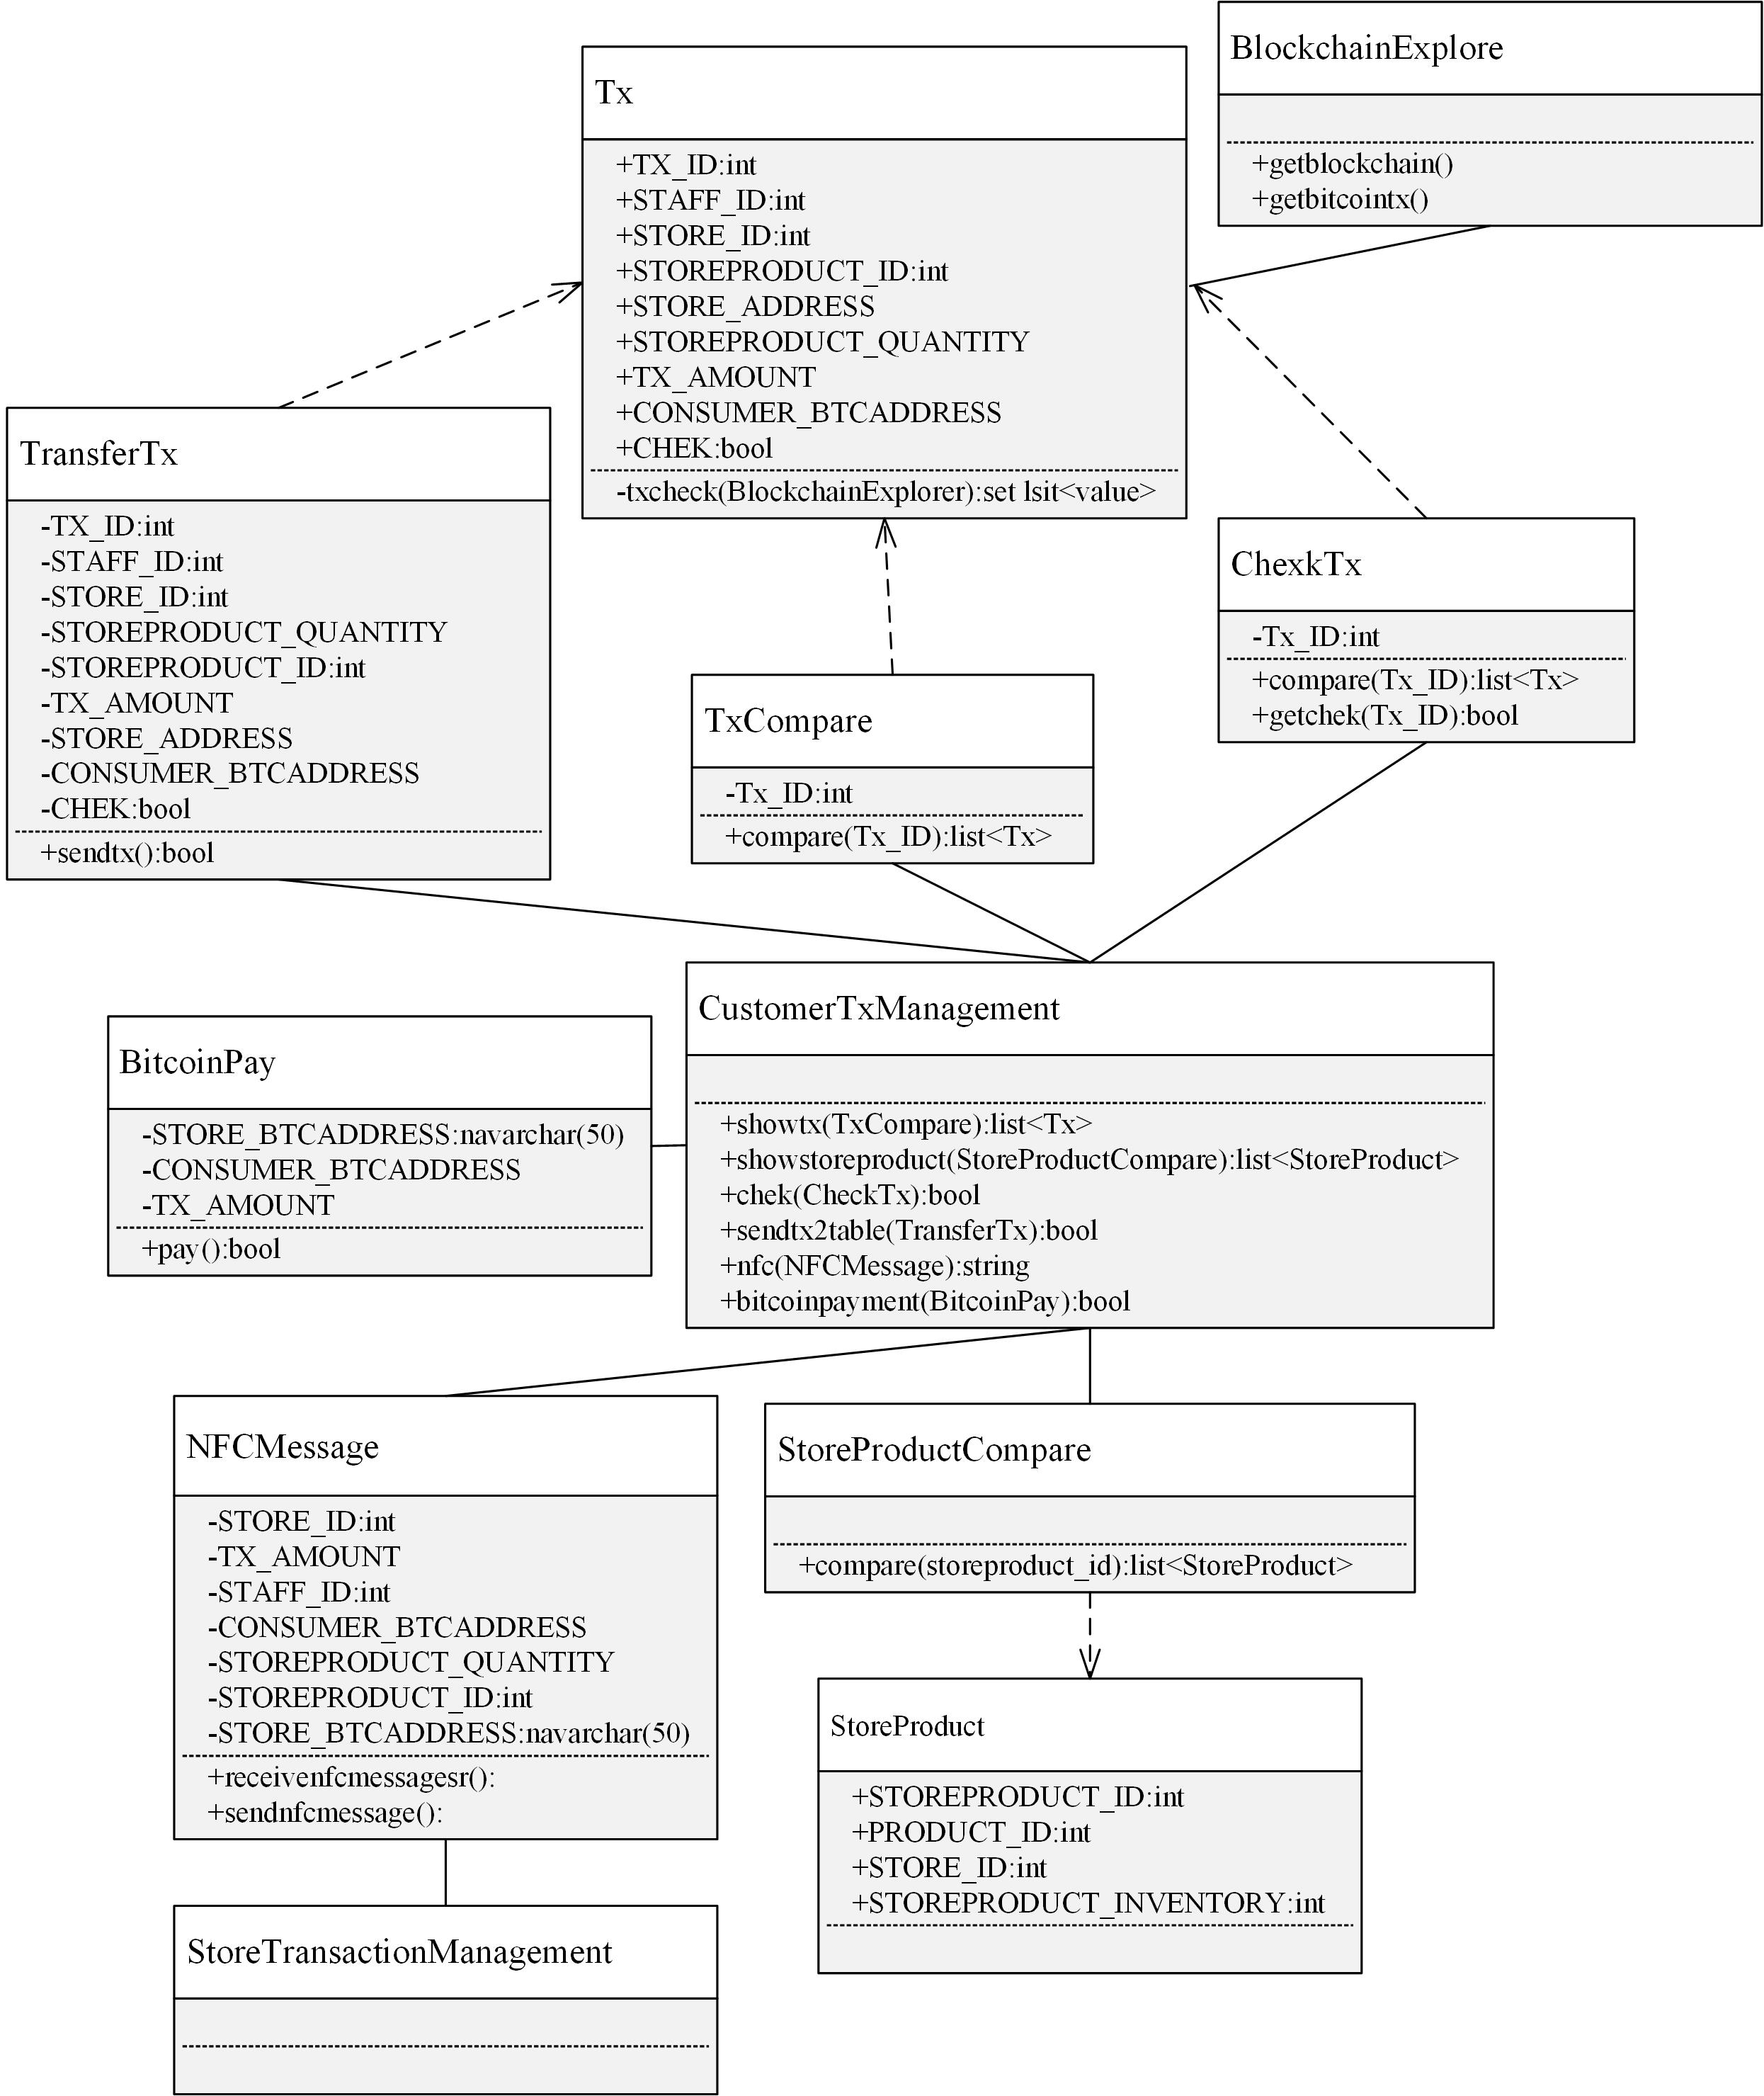
\includegraphics[width = 0.9\textwidth]{c4.jpg}
		\caption{顧客交易管理模塊類圖}\label{c4}
	\end{figure}

	

	圖\ref{time5}為顧客交易管理時序圖,以下為流程說明:

	\begin{figure}[!htbp]
		\centering
		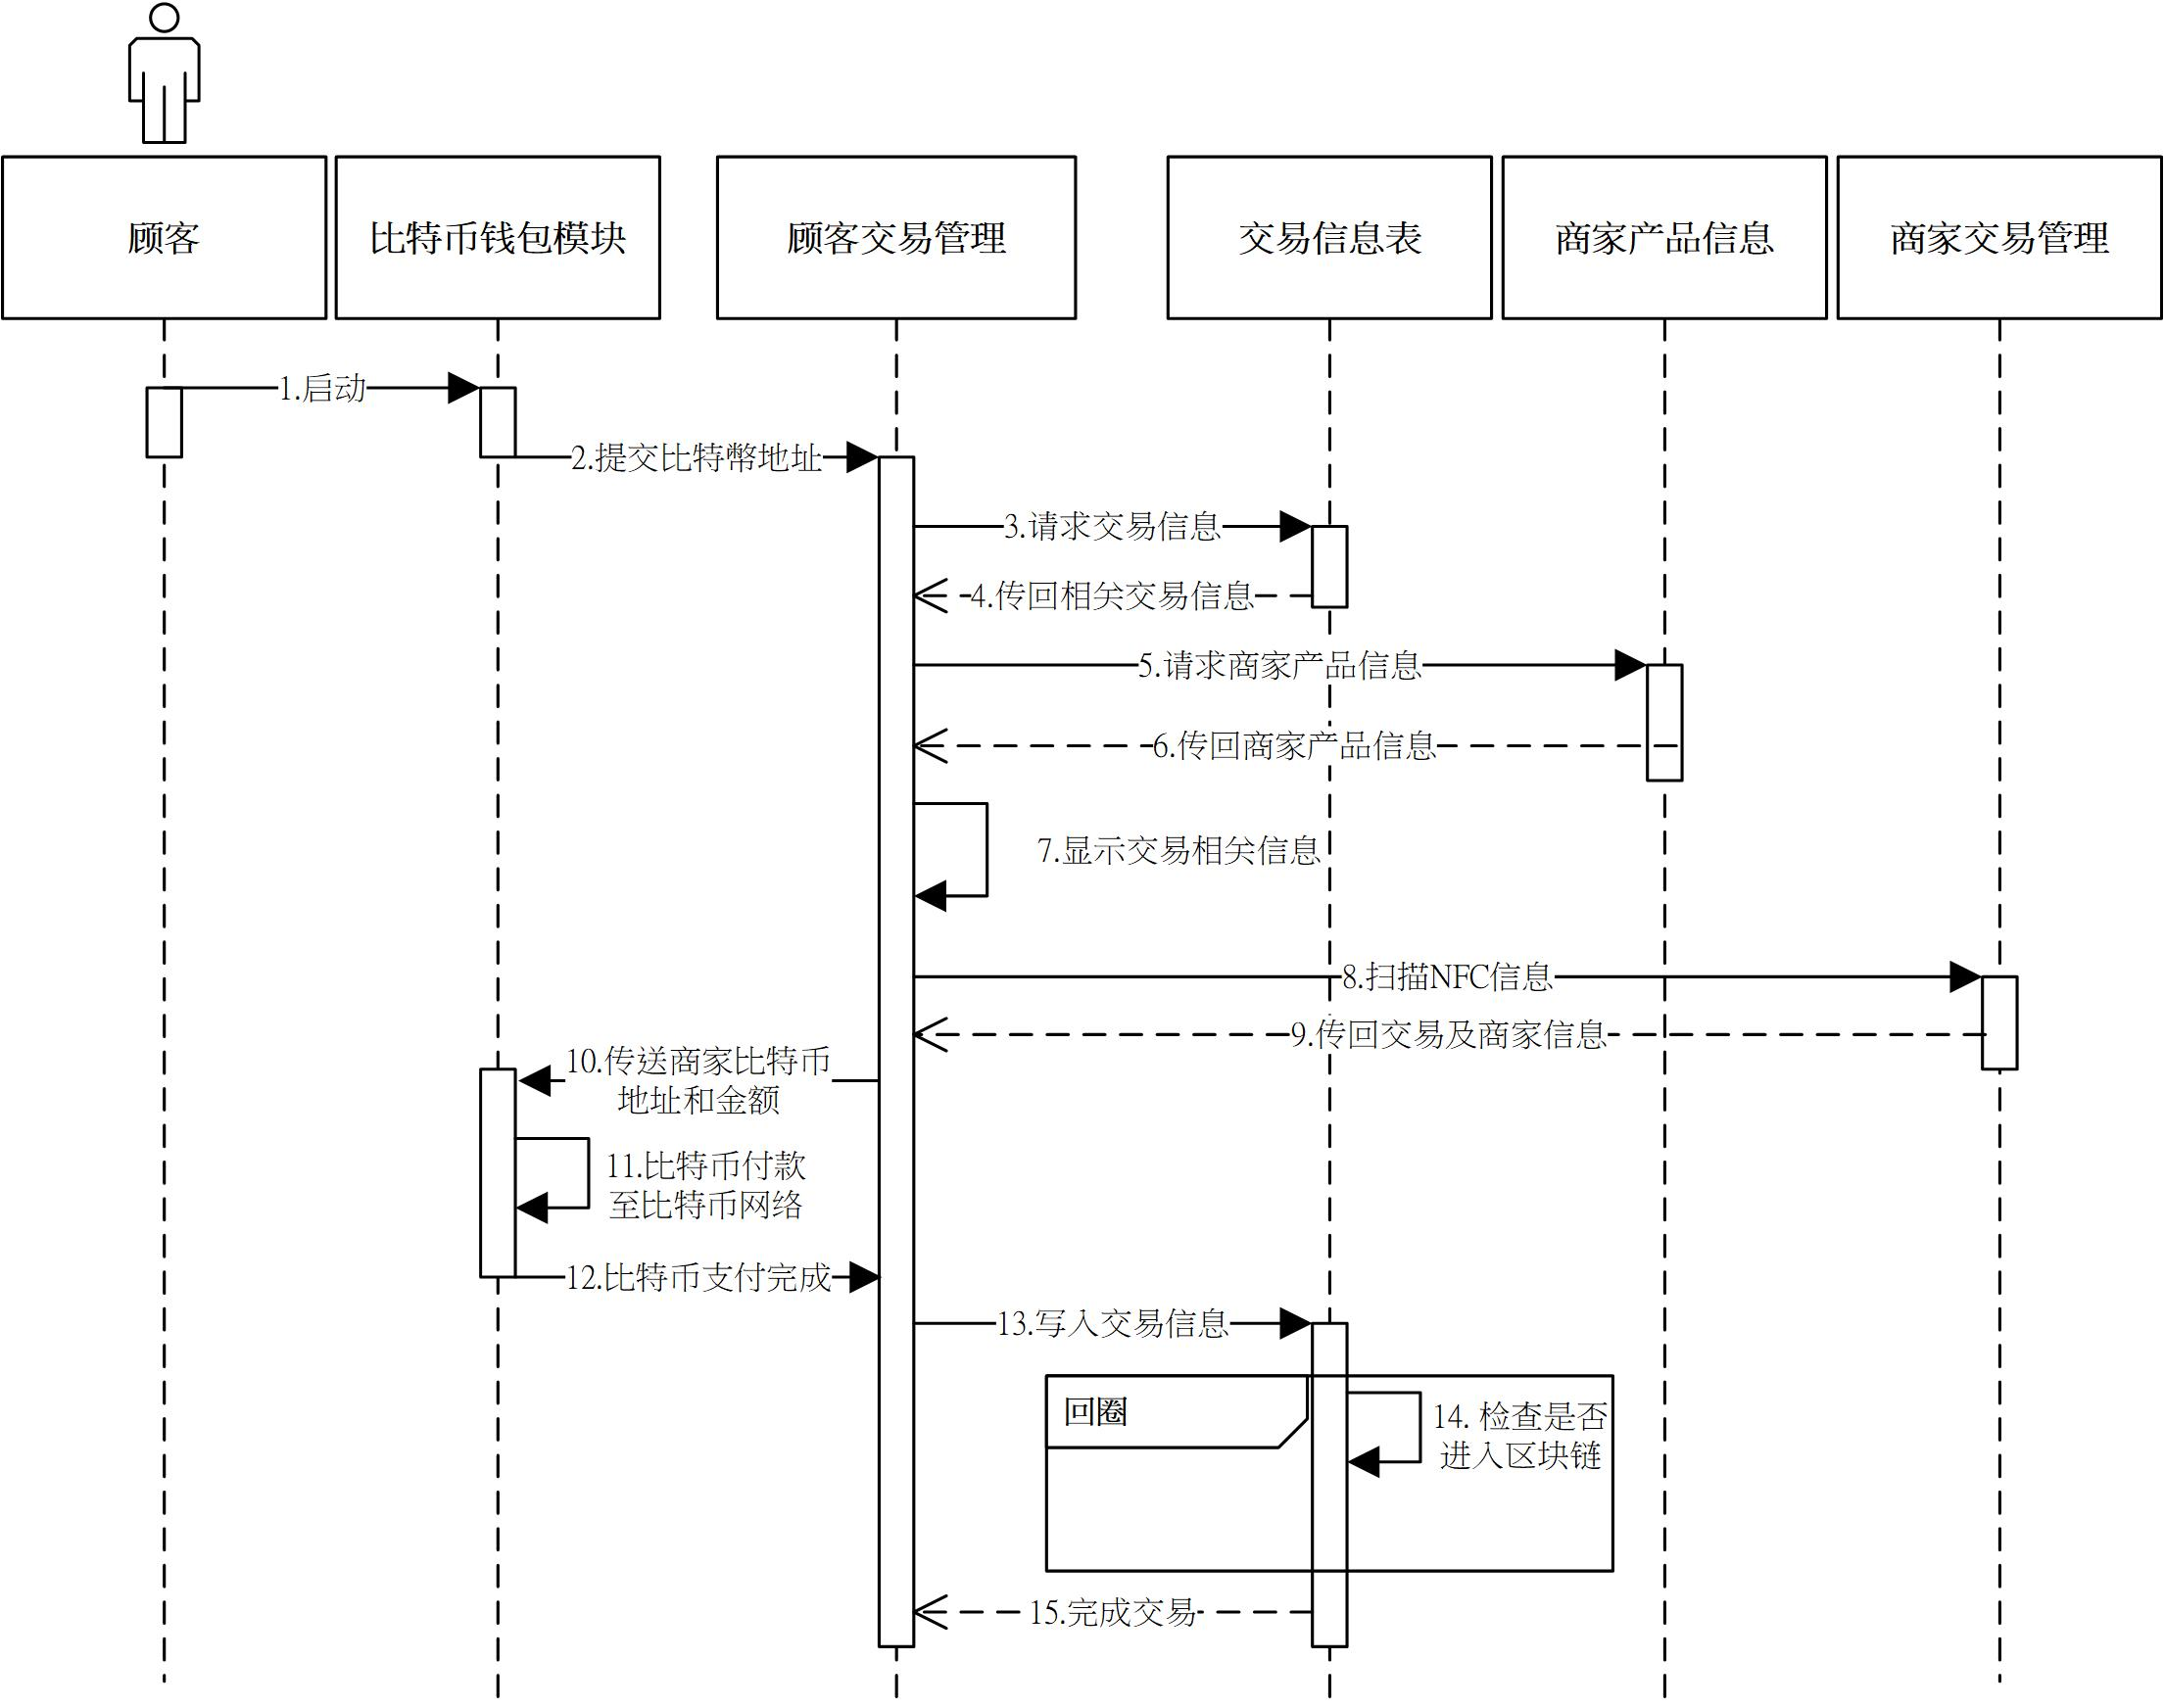
\includegraphics[width = 1\textwidth]{time5.jpg}
		\caption{顧客交易管理時序圖}\label{time5}
	\end{figure}

	\begin{enumerate}
		\item 顧客啟動比特幣錢包管理模塊,屆時比特幣錢包管理模塊再同步最新的區塊鏈信息至手機本地端,並將與手機本身存在的比特幣地址進行核對。
		\item 將所有在比特幣錢包模塊的地址提交到顧客交易管理模塊。
		\item 顧客交易管理模塊將所有拿到的比特幣地址發送到交易信息表,請求完整的交易信息內容。
		\item 交易信息表將概要的交易信息傳回顧客交易管理,此時的交易信息並非相當完整,只有商家產品編號。
		\item 為了使得交易信息更加的完整可以顯示更多的商家產品說明,便將手機本地端數據庫存在的商家產品編號向商家產品信息表提出請求更詳細的說明。
		\item 商家產品信息表傳回詳細的商家產品信息到顧客交易管理模塊。
		\item 顧客交易管理模塊將收到的信息顯示在畫面上。
		\item 當顧客前往商家時,商家掃描完所有顧客欲購買的商家比特幣地址、商家商品、數量、價格以及應付金額之後,便向商家交易管理啟動NFC準備等待顧客的手持裝置進行信息傳輸,此時的顧客將手持裝置與商家手持裝置靠近。
		\item 商家管理模塊透過NFC將交易清單信息傳送到顧客交易管理模塊。
		\item 在商家交易管理模塊重送的交易清單信息當中,包括商家的比特幣地址信息與應付金額,此時顧客交易管理模塊將比特幣地址信息傳送到比特幣錢包模塊。
		\item 在比特幣錢包模塊當中使用secp256k1算法簽署比特幣交易信息,並將交易信息廣播到比特幣網路當中,此時該筆交易信息會進到⽐特幣網絡中的交易緩存等待礦工解出工作量證明的問題,將該筆交易信息存儲到比特幣區塊鏈。
		\item 在完成比特幣簽名後,會生成比特幣的交易哈希值,比特幣錢包管理模塊將比特幣交易哈希值傳送到顧客交易管理模塊。
		\item 顧客交易管理模塊請求交易信息表將比特幣交易哈希值寫入。
		\item 完成寫入後,交易信息表模塊會調用比特幣區塊鏈檢視器的相關函數,不斷檢查該筆比特幣交易是否已經從未確認交易轉變成已確認交易。倘若發現已經確認,則將交易信息表中CHECK欄位的信息從"0"修改為"1"。
		\item 發現交易信息中的CHECK值為"1"之後,便發送完成交易的信息到顧客交易管理模塊。
	\end{enumerate}

	圖\ref{c6}為BRTMS中的顧客Government Green Address交易管理模塊類圖,以下將說明採用Government Green Address與未採用Government Green Address技術的顧客交易管理類圖設計之間的差異。於Tx類中添加ggatxcheck()方法,該方法可以不斷檢查交易信息表中的交易是否來自Government Green Address地址,倘若是則不需要等待區塊鏈的驗證時間可以即刻認定該筆交易為有效,快速提交比特幣交易速度。GovernmentGreenaddressCheck類中compare()方法是為了查找與TX\_ID相符的交易信息,getchek()方法則是向交易信息表中詢問符合TX\_ID的交易信息是否已經被修改為"1"。其中GovernmentGreenaddressBitcoinPay類中的multiplesignature()方法可以實現多重簽章算法,使得本系統可以支持即時交易。governmentgreedaddresspay()方法是將多重簽章算法廣播報導比特幣網路。


	\begin{figure}[!htbp]
		\centering
		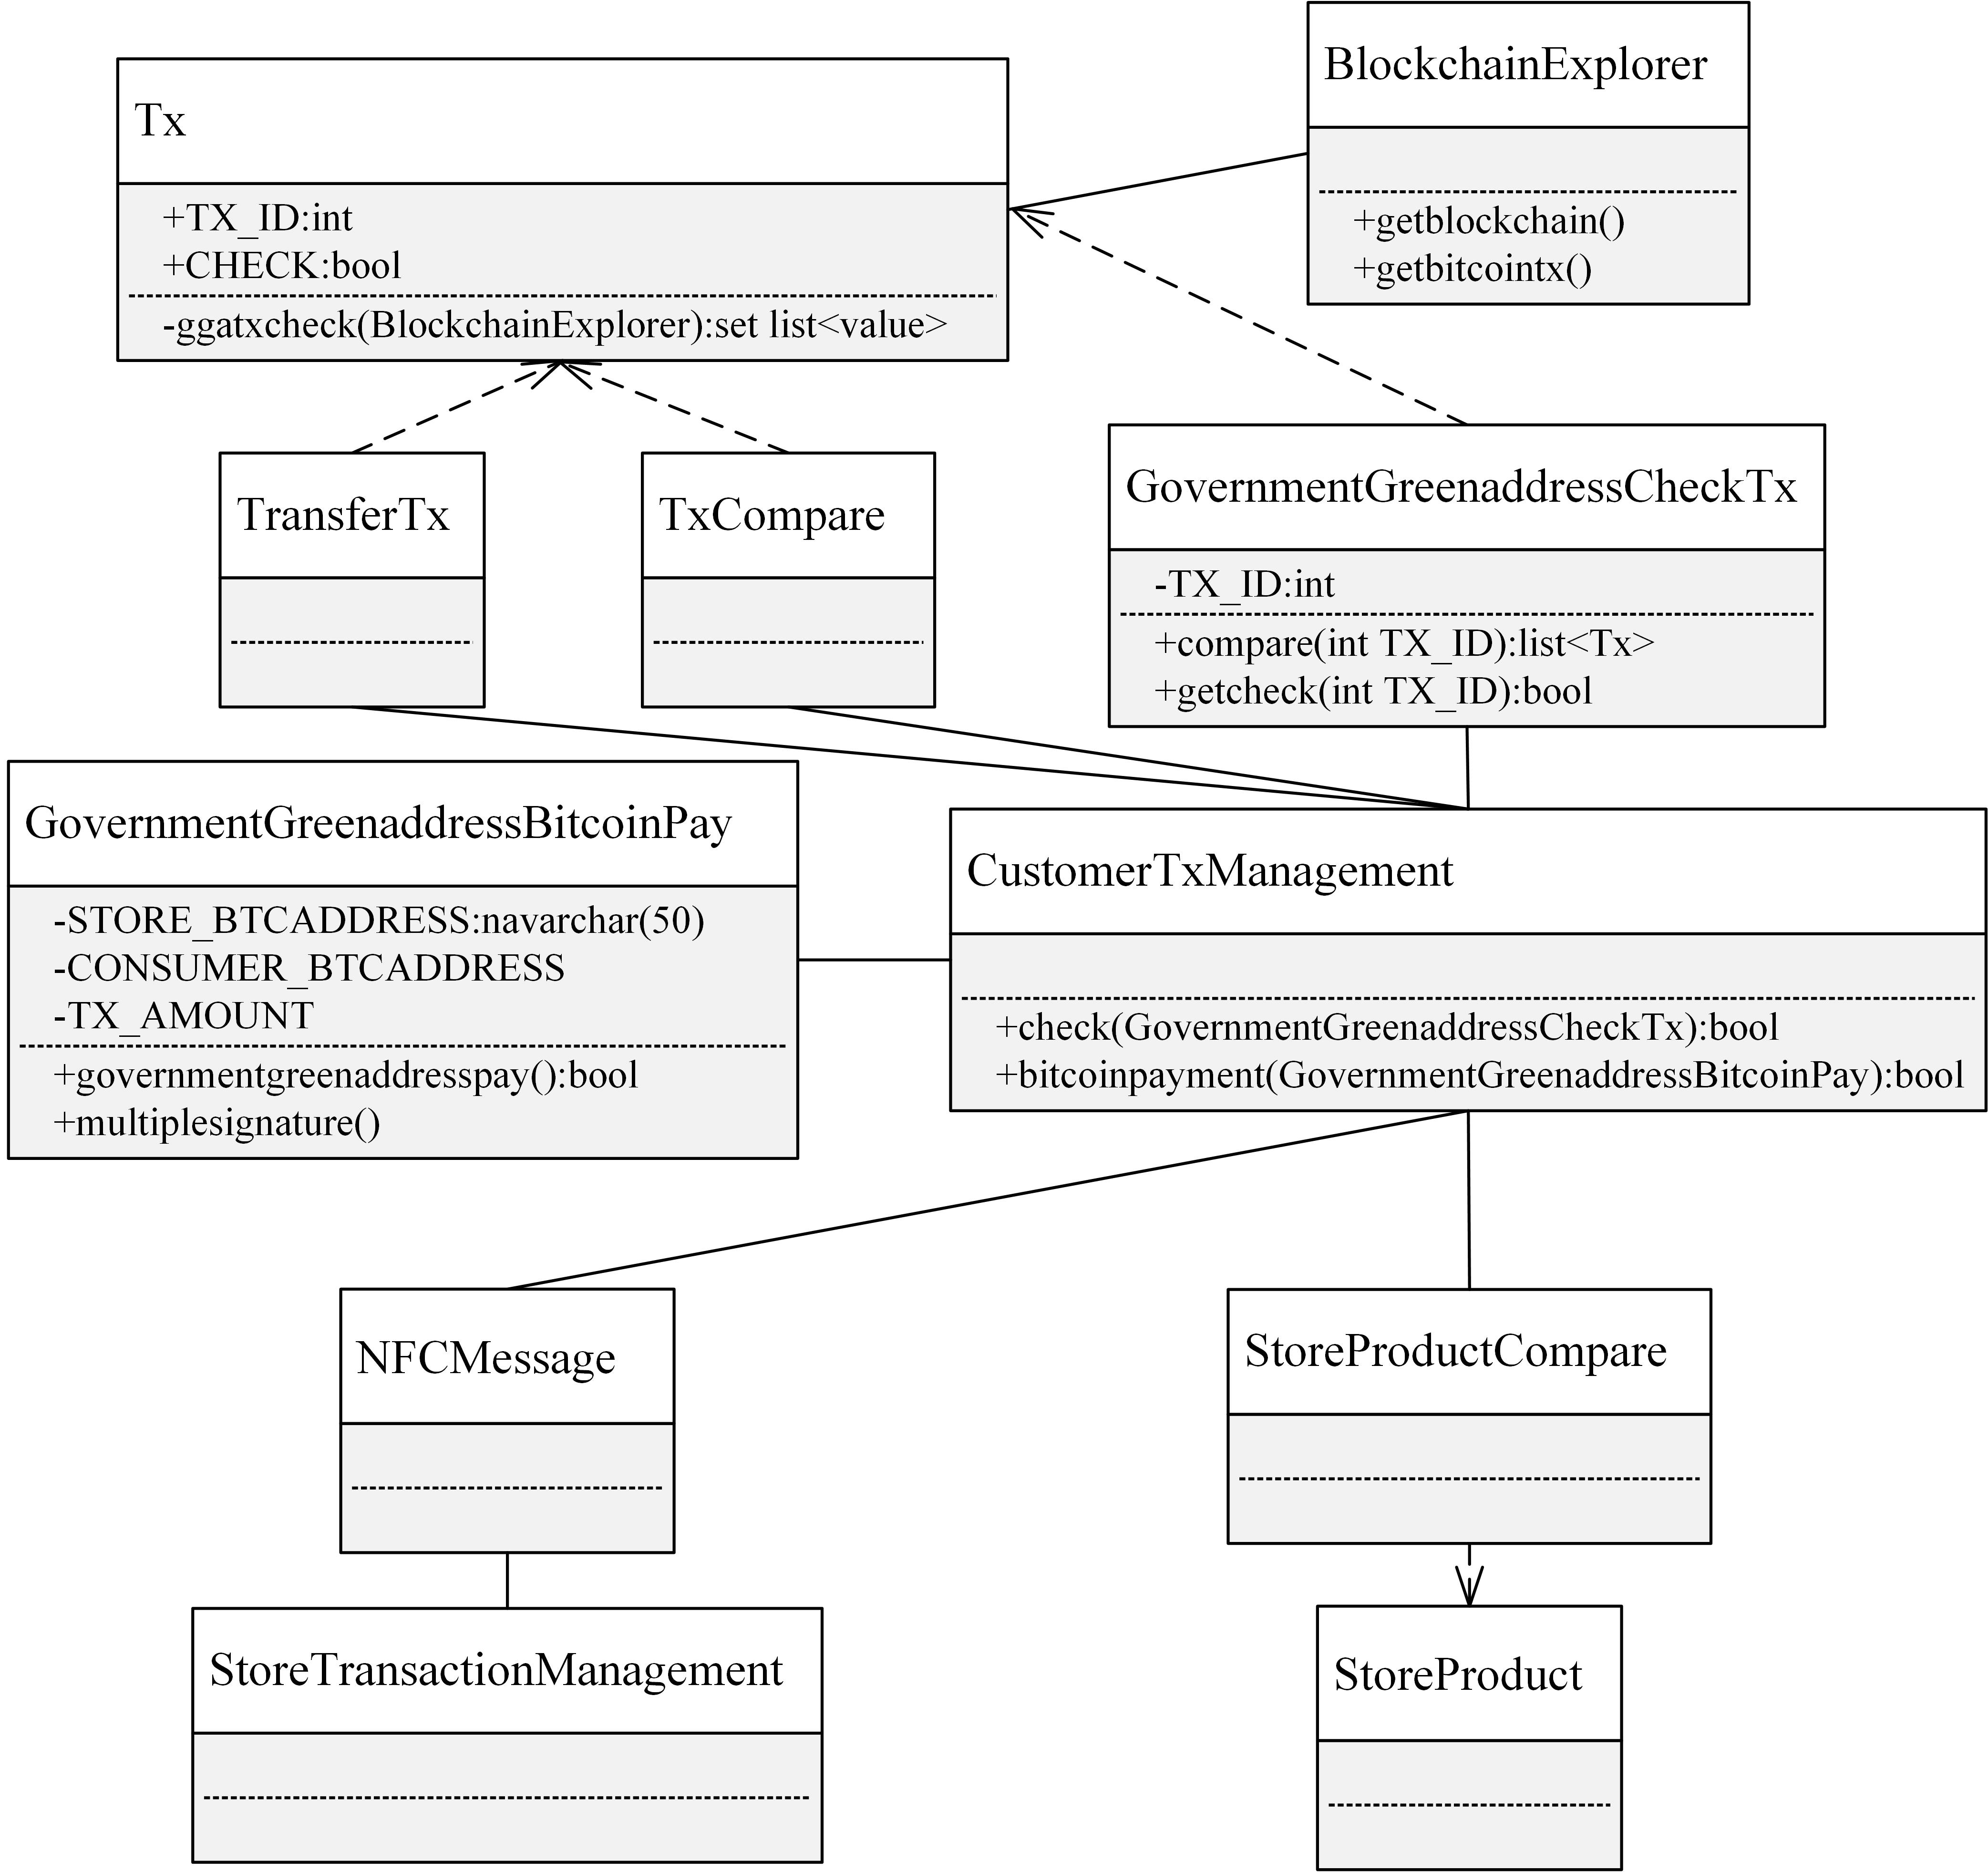
\includegraphics[width = 0.6\textwidth]{c6.jpg}
		\caption{顧客Government Green Address交易管理模塊類圖}\label{c6}
	\end{figure}

\section{系統實現}

% \section{區塊鏈的實名交易監督系統實現}

為了驗證和證明所提議的BTMS用於比特幣支付收款監督的可行性和有效性,將其運行在用於商家商品管理和維護的Java應用程序的SMIMSS子系統,用於商家職工的運行在Android App上的SMCTSS以及運行在App上的用於顧客的CMPTSS。
如圖\ref{fig5}所示,SMIMSS 的 Java應用程序可以幫助商家登錄到系統或創建一個新帳戶。 授權商家成功登錄系統後,商家可以插入或更新產品列表,如圖\ref{fig6}所示。實現的SMIMSS Java應用程序執行前面部分中所述的功能。

\begin{figure}[!htbp]
	\centering
	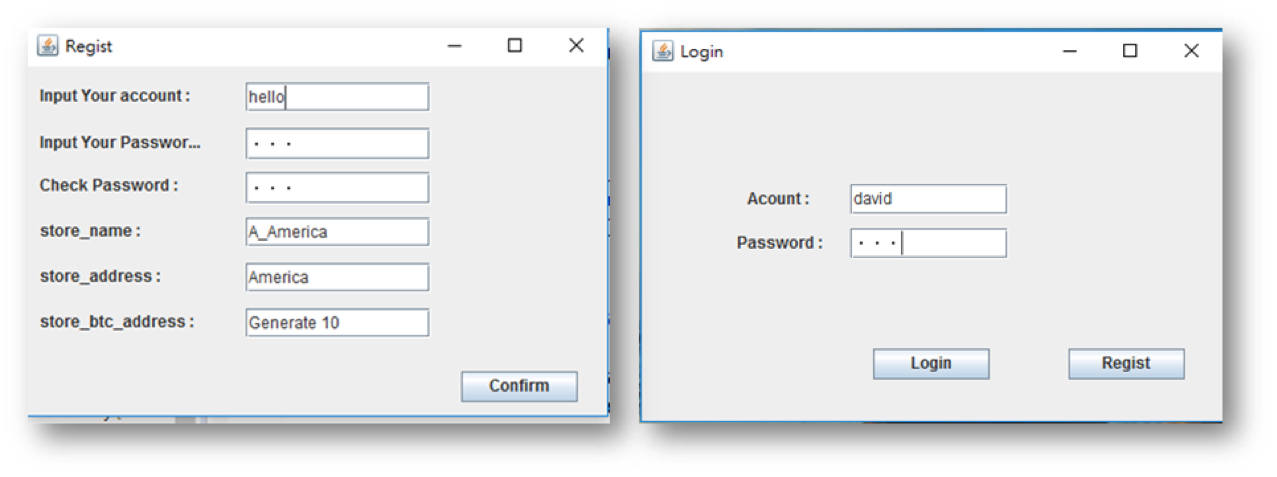
\includegraphics[width = 0.9\textwidth]{fig5.png}
	\caption{SMIMSS的Java應用程序的註冊和登錄界面}\label{fig5}
\end{figure}

\begin{figure}[!htbp]
	\centering
	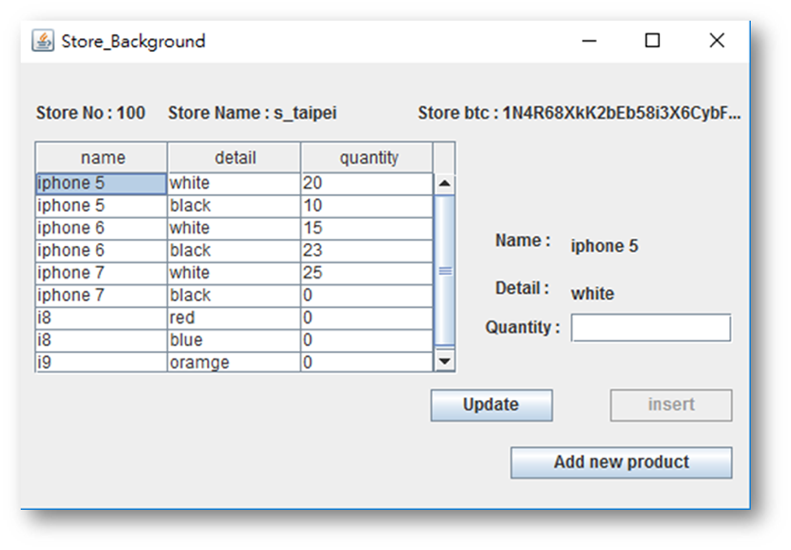
\includegraphics[width = 0.6\textwidth]{fig6.png}
	\caption{在SMIMSS中插入或更新授權商家的產品目錄}\label{fig6}
\end{figure}

商家的產品信息可以通過RFID標籤掃描,存儲到雲端數據庫中,商家職工可以使用實現的SMCTSS Android客戶端,啟用NFC監聽器,從購物車中的顧客購買產品中讀取RFID標籤信息。 在如圖\ref{fig7}所示的第一項活動中,商家職工必須登錄才能獲得授權訪問SMCTSS功能。 然後,在第二項活動中,SMCTSS應用程序可以通過使用SMIMSS中應用的雲數據庫檢查產品RFID標籤信息並將其展示給顧客,從而將掃描的產品列入購物車。 在圖\ref{fig7}的第三項活動中,顧客可以要求職工刪除購買物品以,並確認最終交易清單。 最後,SMCTSS應用程序將自動使用比特幣測試網絡(Bitcoin Testnet)\supercite{bitcointestnet}幫助職工確認發布此比特幣交易的收款人地址,如圖\ref{fig7}所示。    

\begin{figure}[!htbp]
	\centering
	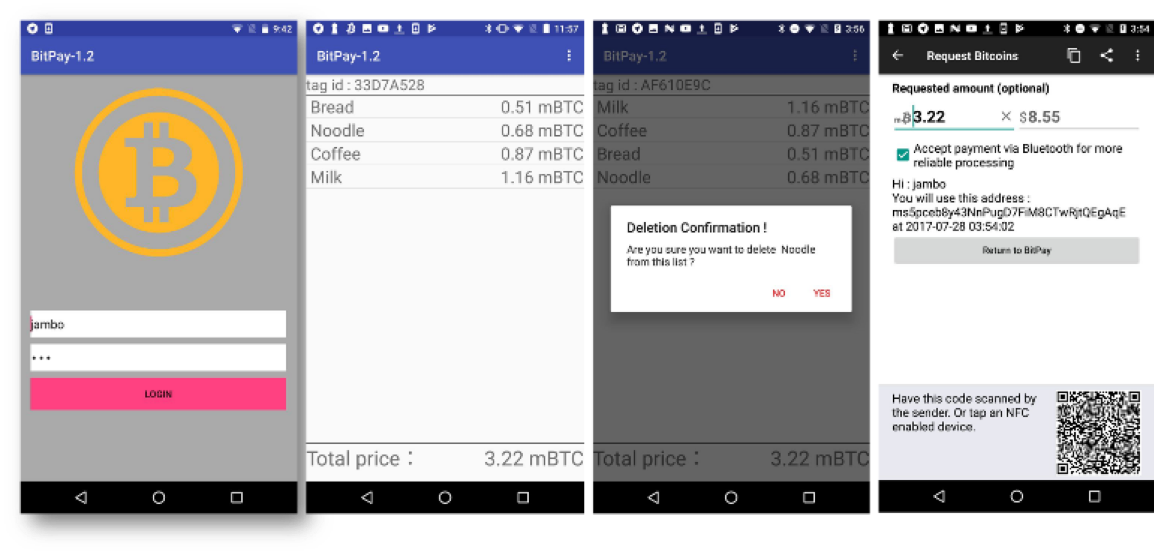
\includegraphics[width = 1\textwidth]{fig7.png}
	\caption{登錄、等待結帳的商品、刪除商品及支付確認}\label{fig7}
\end{figure}

同時,顧客將使用與SMCTSS App相對應的CMPTSS Android App通過比特幣完成採購產品交易。 如圖\ref{fig8}所示,第一個活動表示顧客確認購買產品創建交易數據庫的交易清單,第二個活動顯示包括金額和付款人比特幣地址在內的付款確認,第三個活動顯⽰該錢包交易的歷史記錄,凡是出入該錢包的所有交易都會被顯示出來,
錢包可以同時作為買⽅和賣⽅,最後在第四項活動中顯示了該筆交易詳細採購產品的交易憑據。    

\begin{figure}[!htbp]
	\centering
	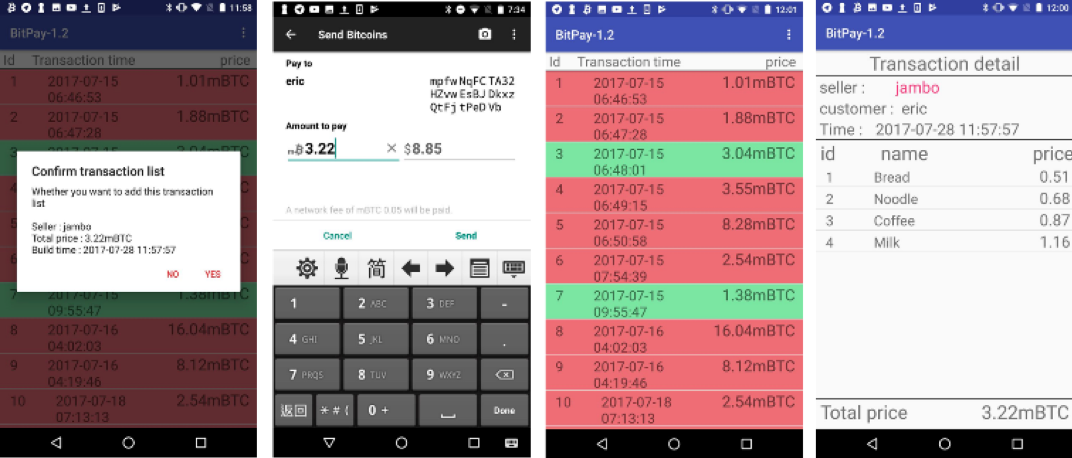
\includegraphics[width = 1\textwidth]{fig8.png}
	\caption{在CMPTSS App中,交易確認,付款確認、交易歷史記錄和發票}\label{fig8}
\end{figure}